\chapter{Building Adaptive Hybrid Representations}\label{chap:method}
% ---- TAKEAWAYS ----
% - Joining whole representations adds their irrelevant features along with the useful ones. The hybrid combines and filters at once.
% - A hybrid is an input, not a model: up to a budget of features, selected from several base representations by a search for one dataset and one downstream model.
% - No setting of the search wins on every dataset or model, so importance method, allocation method, representation count, internal evaluator, budget and downstream model are all searched.
% - Every selected feature traces back to its representation, so a blueprint can show a chemist which substructures and descriptors the model relies on.
% - The method needs only a supervised label and several vector representations of the same samples, so it carries over to antibodies, reactions, nucleotides and tumor data.
% - Where one representation already dominates, the hybrid should show little gain. The search is costly and must be rerun when the data, representations or model change.
% ---- END TAKEAWAYS ----

% [TRIM3 2026-09-30] simplified
% CODE INPUT
% TODO: review, needs manual review
This chapter asks how several representations can be joined without also joining their irrelevant features. Our answer is the adaptive hybrid representation, a set of at most a fixed number of features, the budget, selected from several base representations by a search for one dataset and one downstream model. The search covers the importance method, the allocation method, the number of representations, the internal evaluator, the budget and the downstream model. Because every selected feature traces back to its representation, each search yields a blueprint that records where its features came from, and names them where the base representation has named features. We test the method on small molecules, antibodies, reactions, nucleotide sequences and tumor data. In preliminary runs on hERG $K_i$ with one default configuration, the hybrid had a lower RMSE than the best single representation with SVM and LightGBM on all three folds and was level with it for random forest.


% TODO: how do I reference these properly? 
\section{Introduction}
% [notes moved to thesis_notes_moved.md]

% [TRIM3 2026-09-30] simplified
% [TRIM 2026-09-30] shortened
% CODE INPUT
% TODO: review, needs manual review
Chapter~\ref{chap:flaws} showed that standard representations carry many features that do not vary, or do not matter, on a given dataset, and that distances over all features inherit the problem. It called for features chosen for the task from several representations, with the irrelevant ones removed. Chapter~\ref{chap:robustness} showed that the best representation changes with both the dataset and the model, a reason to search over this choice rather than fix it.

% [TRIM 2026-09-30] shortened
% CODE INPUT
In this chapter we build the adaptive hybrid representation, hereafter the hybrid, and report first results on when and why it helps. The questions this chapter and Chapter~\ref{chap:similarity} address are set out in Chapter~\ref{chap:intro} (Section~\ref{sec:intro:hybrid_questions}).

% [TRIM3 2026-09-30] simplified
% [TRIM2 2026-09-30] removed the 'methods are final' caveat, the 5-outer-folds statement and the two RESULT NEEDED placeholders that repeat the chapter opening
% CODE INPUT
% TODO: review, needs manual review
This chapter measures prediction, including prediction under label noise. Distances in a hybrid, noise detection and learning with noisy labels are covered in Chapter~\ref{chap:similarity}.

% [TRIM3 2026-09-30] paragraph removed
% CODE INPUT


\subsection{Combining Representations and the Alternatives}
% [notes moved to thesis_notes_moved.md]
% - TODO(lit): read the Turkina2025 full text for whether a fixed number of bits is kept per fingerprint, or all bits are ranked together.

% [TRIM3 2026-09-30] simplified
% TODO: review
% TODO: review, needs manual review
Conjoint fingerprints predicted binding affinity better than their component fingerprints across a range of models \citep{Xie2020}. Adding bioactivity-based fingerprints to structure-based ones like ECFP4 improved both predictive performance and scaffold-hopping \citep{Laufktter2019}. Features selected from six non-hashed fingerprints and combined by feature importance score within individual models consistently improved predictive accuracy over the original fingerprints \citep{Turkina2025}.

% [TRIM 2026-09-30] paragraph removed, text in cuts file

% [TRIM3 2026-09-30] simplified
% [TRIM 2026-09-30] shortened
% TODO: REVIEW MODIFICATION
% TODO: review, needs manual review
Most of this work combines standard fingerprints and linear representations like SMILES \citep{Xie2020, Laufktter2019}. We also include GNN embeddings, since graph-based representations capture structural information that fingerprints often lose. We extend how feature importance is computed and how features are selected and joined, and we test augmentation, adding small sets of structural features to one base representation.

% TODO: review and the li and deng defini
% [TRIM 2026-09-30] paragraph removed, text in cuts file

% [TRIM3 2026-09-30] simplified
% [TRIM 2026-09-30] \citep{Beaude2025} carried over from the removed older version, whose inline note read: TODO: REVIEW MODIFICATION -- was \citep{Zhang2024}, which had no bibliography entry and no known source. CrossAttOmics (Beaude et al. 2025) is a verified cross-attention intermediate-fusion paper. Swap it if you meant a different paper.
% TODO: REVIEW MODIFICATION
% [RESTORE 2026-09-30] Ch5a-8
% TODO: review, needs manual review
Concatenation, the most common strategy, needs only one downstream model but degrades when the feature sets are not homogeneous \citep{Stahlschmidt2022}. It also obscures which representation is responsible for the score. Deng et al.\ found that appending RDKit2D descriptors to GROVER lowered RMSE on 9 of 24 datasets, yet called the practice ``misleading'' for measuring the contribution of individual representation types \citep{Deng2023}. Late fusion trains one model per source and aggregates the predictions \citep{Steyaert2023}, which avoids the dimensionality problem but loses interactions between sources. Intermediate fusion keeps them (MOGONET \citep{Wang2021}, cross-attention \citep{Beaude2025}) but must be retrained from scratch to add a source. Multiple kernel learning \citep{Gonen2011, Cichonska2018} works only with kernels and yields no interpretable feature subsets. There is no decisive evidence that any of these strategies is broadly superior \citep{Steyaert2023}.

% [TRIM 2026-09-30] paragraph removed, text in cuts file

% [TRIM3 2026-09-30] simplified
% TODO: REVIEW MODIFICATION
% TODO: review, needs manual review
In practice, most groups default to one representation, and few combine representations beyond concatenation. Concatenating ECFP4 (2,048 features), MHG-GNN (1,024) and Mordred descriptors (1,613) gives about 4,700 features, while a dataset may contain only a few hundred labeled samples. At such ratios, more features mean worse predictions \citep{Hughes1968, Bellman1961}. A concatenation of two representations scored between its two parts, rather than above the better one, on \textbf{[RESULT NEEDED: count of datasets]}. We propose that this is because concatenation adds the irrelevant features of both parts along with the useful ones, so a method that joins representations has to combine and filter at the same time.

% [TRIM 2026-09-30] paragraph removed, text in cuts file

% [TRIM3 2026-09-30] simplified
% TODO: REVIEW MODIFICATION
% [RESTORE 2026-09-30] Ch5a-9
% TODO: review, needs manual review
New models keep appearing, well beyond small molecules; a recent review counted over 40 molecular foundation models published between 2020 and 2024 \citep{Song2026}. A new downstream model may prefer a different feature set, and it therefore receives its own search. A new model's frozen embeddings enter as one more base representation without any change to the method.

% [TRIM3 2026-09-30] simplified
% TODO: review, needs manual review
% [RESTORE 2026-09-30] Ch5a-1
In a comparison of 62,820 models on molecular property prediction benchmarks, RDKit2D descriptors matched or outperformed learned features from graph neural networks and pretrained language models on the majority of datasets \citep{Deng2023}. Descriptor-based models held 73\% of top-three positions on 11 benchmarks \citep{Jiang2021}. In 1,310 ChEMBL assays, feedforward networks on ECFP fingerprints outperformed graph convolutions and SMILES-based recurrent models \citep{Mayr2018}. The choice of input changes the result substantially, yet no single representation wins, and there is no systematic way to exploit this. No single protein language model is consistently best on all tasks \citep{Kenlay2024, Schmirler2024}, and no pathology foundation model dominates on clinical endpoints \citep{ElNahhas2025}.

% [TRIM 2026-09-30] paragraph removed, text in cuts file

% [TRIM3 2026-09-30] simplified
% TODO: REVIEW MODIFICATION
% TODO: review, needs manual review
The representations used in this thesis are listed in Tables~\ref{tab:reps_smallmol}, \ref{tab:reps_reactions}, \ref{tab:reps_antibodies}, \ref{tab:reps_nucleotides} and~\ref{tab:reps_tcga}.

% [TRIM2 2026-09-30] older concatenation/CASH paragraph (with the Tishby2015 information-bottleneck argument) removed, text in cuts2 file

% [TRIM3 2026-09-30] simplified
% TODO: REVIEW MODIFICATION
% TODO: review, needs manual review
The hybrid search keeps individual original features from several base representations, so its selection spans representation boundaries. Its closest analogy is perhaps the combined algorithm selection and hyperparameter optimization (CASH) problem \citep{Thornton2013}, to which it adds a third choice, namely which features from which representations enter the model.

% TODO: background on feature selection algorithms
% But more of a direct focus on feature selection

% TODO: background on PCA and other dimensionality reduction techniques


% [TRIM3 2026-09-30] simplified
% CODE INPUT
% TODO: review, needs manual review
Ensembling fits one model per representation and pools their predictions, combining representations after prediction rather than before. Consensus QSAR works this way \citep{Valsecchi2020}, so it cannot exploit cases where one representation's noise is another's signal. No model in an ensemble sees features from two representations together, and every representation and every model must be computed for each new molecule.

% [TRIM3 2026-09-30] simplified
% CODE INPUT
% TODO: review, needs manual review
Feature selection keeps a subset of the original features, unlike principal component analysis (PCA), which builds new ones. Of its three families \citep{Guyon2003}, filter methods score features against the labels before any model is fitted, as minimum-redundancy maximum-relevance selection (mRMR) ranks features by their mutual information with the label minus their redundancy with features already chosen \citep{Peng2005}. Wrapper methods score subsets of features by fitting the model \citep{Kohavi1997}. Embedded methods select features while the model is fitted, as the lasso does \citep{Tibshirani1996}. Recursive feature elimination fits a model, drops the lowest-ranked features and repeats \citep{Guyon2002}.

% [TRIM3 2026-09-30] simplified
% [TRIM 2026-09-30] shortened
% CODE INPUT
% TODO: review, needs manual review
The hybrid ranks features by a fitted model's importance scores, as embedded methods do, and keeps a fixed number of the top-ranked ones, as a filter does. Classical methods treat all features as one flat list. The nearest classical relative, the group lasso, keeps or drops predefined groups of variables whole \citep{Yuan2006}, whereas the hybrid splits the budget among representations (Section~\ref{sec:method:allocation}). Because only original features are kept, each traces back to one representation, which makes blueprints possible.

% [TRIM3 2026-09-30] simplified
% [TRIM2 2026-09-30] cut the kernel PCA / t-SNE / UMAP sentence
% CODE INPUT
% [RESTORE 2026-09-30] Ch5a-7
% TODO: review, needs manual review
PCA replaces the original features with fewer linear combinations of them, ordered by the variance they explain \citep{Jolliffe2016}. Its components usually depend on all the original features, so they are hard to interpret, and they depend on feature units unless each feature is z-scored first \citep{Jolliffe2016}. This matters when fingerprint bits, descriptors and embeddings are joined. PCA never sees the labels, and components with small variance can still predict the property \citep{Jolliffe1982}. Partial least squares (PLS), the supervised counterpart in chemometrics, builds components that covary with the property \citep{Wold2001}. Neither gives components that can be traced to one substructure, descriptor or representation, so no blueprint can be read from them.

% [TRIM3 2026-09-30] simplified
% CODE INPUT
% TODO: review, needs manual review
Of the alternatives above, PCA, PLS and feature selection also reduce the number of features, but models may want different numbers of features and different features. Distance-based models such as $k$-nearest neighbors (kNN) and SVM use every feature in every distance (Chapter~\ref{chap:flaws}), whereas tree ensembles choose one feature per split and can partly ignore irrelevant ones. Dablander suggests that using the labels may add a risk of overfitting \citep[p.~138]{Dablander2024}, and Sort \& Slice, which uses no labels, outperformed two label-based schemes for selecting substructure features \citep{sns}. Table~\ref{tab:hybrid_alternatives} compares these alternatives with the hybrid.

% [TRIM3 2026-09-30] simplified
% CODE INPUT
% TODO: review, needs manual review
\begin{table}[htbp]
\centering
\small
\setlength{\tabcolsep}{3pt}
\begin{adjustbox}{max width=\textwidth,max totalheight=0.78\textheight}
\begin{tabular}{P{4.2cm}P{2.3cm}P{2.1cm}P{2.3cm}P{2.6cm}}
\toprule
Method & Uses the labels & Keeps original features & Several representations & Retrain to add one \\
\midrule
Concatenation \citep{Stahlschmidt2022} & no & yes & yes & yes \\
Late fusion and ensembling \citep{Steyaert2023, Valsecchi2020} & only if pooling weights are learned & yes & no & no, one more model \\
Intermediate fusion \citep{Wang2021} & yes & no & yes & yes \\
Multiple kernel learning \citep{Gonen2011, Cichonska2018} & yes & no, kernels only & yes & yes \\
PCA and PLS \citep{Jolliffe2016, Wold2001} & PCA no, PLS yes & no & yes, on a concatenation & yes \\
Flat feature selection \citep{Guyon2003} & yes & yes & yes, on a concatenation & yes \\
Group lasso \citep{Yuan2006} & yes & yes, whole groups & yes & yes \\
Adaptive hybrid representation & yes & yes & yes & search rerun, method unchanged \\
\bottomrule
\end{tabular}
\end{adjustbox}
% [RESTORE 2026-09-30] Ch5a-14
% TODO: review, needs manual review
\caption[Methods for combining or reducing representations.]{Methods for combining or reducing representations, compared by whether they use the labels, keep the original features, let one model see several representations, and must refit to add a representation.}
\label{tab:hybrid_alternatives}
\end{table}
\subsection{The Adaptive Hybrid Representation}
% [notes moved to thesis_notes_moved.md]

% TODO: is this right??? I'm making shit up with NGBoost.
% [TRIM 2026-09-30] paragraph removed, text in cuts file

% [TRIM4 2026-09-30] NGBoost R^2 and robustness numbers cut; pointer to Chapter robustness kept. Text in cuts4 file
% [TRIM3 2026-09-30] simplified
% TODO: REVIEW MODIFICATION
% TODO: Ch3 update -- waits for the new Chapter 3 results. Once they are in, say here what Chapter 3 shows about NGBoost on clean labels (which representation it did best on), or drop the pointer.
% TODO: review, needs manual review -- Ch3 update applied 2026-09-30: NGBoost facts taken from the new Chapter 3 (QM9, Gaussian noise; Chapter 3 limitations paragraph).
One approach rarely suits every problem. On QM9 in Chapter~\ref{chap:robustness}, NGBoost had the lowest predictive performance on clean labels on four of the six representations, yet with PDV it was the most robust model and had the highest predictive performance at the highest noise level.

% [TRIM2 2026-09-30] signed-off original 'But as important as...' removed; the rewrite 'Selecting useful features matters...' below is kept. Text in cuts2 file

% [TRIM3 2026-09-30] simplified
% [TRIM 2026-09-30] shortened
% TODO: REVIEW MODIFICATION
% TODO: review, needs manual review
Filtering out useless features matters as much as selecting useful ones. Pooling many representations adds irrelevant features that act as noise (Chapter~\ref{chap:flaws}), and in an earlier exploratory study, the noise handling methods that used a distance between molecules performed worst (Section~\ref{sec:lnl_motivation}).

% [TRIM3 2026-09-30] simplified
% CODE INPUT
% TODO: review, needs manual review
Formally, an adaptive hybrid representation is a set of up to a fixed number of features, the budget, selected from several base representations of the same molecules. A search chooses it for one dataset and one downstream model, so a different dataset, split or model gives a different hybrid. The hybrid is an input rather than a model, so any standard supervised model can be trained on it. It is intended for base representations that describe different aspects of the molecule, such as PDV descriptors, ECFP4 bits, graph embeddings and sequence embeddings.

% [TRIM3 2026-09-30] simplified
% [TRIM 2026-09-30] shortened
% CODE INPUT
% TODO: review, needs manual review
The budget is split between the representations before any feature is picked, and each representation's features are ranked only against each other. In a single ranking, a wide representation (thousands of features) can crowd out a narrow one (tens), and importance scores from different types of feature are not on a common scale. One pooled allocation method, the global pool, ranks the features offered by every representation together, so that per-representation and pooled selection are compared instead of assumed.

% [TRIM3 2026-09-30] simplified
% CODE INPUT
% [RESTORE 2026-09-30] Ch5a-11
% TODO: review, needs manual review
A hybrid can also be used to measure similarity in two ways. Distances can be computed in an ordinary hybrid, or the search can pick features by how well each molecule's activity is predicted from its five nearest neighbors. Both are defined in ``Similarity in a hybrid'' (Chapter~\ref{chap:similarity}).


\subsection{Blueprints and Their Chemical Interpretation}
% [notes moved to thesis_notes_moved.md]

% [TRIM3 2026-09-30] simplified
% CODE INPUT
% TODO: review, needs manual review
A finished search is saved as a blueprint, which records the settings needed to rebuild the hybrid. Because each selected feature traces back to its representation and importance rank, the search returns information about the problem as well as a better score. The best configuration is kept for each downstream model and budget, giving one blueprint per pair, so comparing blueprints at one budget shows whether tree ensembles and neural networks draw on different features.

% [TRIM3 2026-09-30] simplified
% CODE INPUT
% TODO: review, needs manual review
Some selected features can be read by a chemist. A PDV descriptor has a name, such as molecular weight or logP, an ECFP4 bit can be shown as the atom environment that sets it, and a MACCS key stands for a known substructure. For an antibody the readable unit is a sequence position and its residue, and for gene expression a named gene set, such as a pathway or a chromosome arm. A feature of a learned embedding shows only which representation was useful, not the chemistry (Chapter~\ref{chap:flaws}).

% [TRIM3 2026-09-30] simplified
% CODE INPUT
% [RESTORE 2026-09-30] Ch5a-12
% TODO: review, needs manual review
Readable features serve two purposes. Substructures or descriptors that recur among the kept features can point to parts of the molecule that may be involved in binding or activity, a starting point for a chemist rather than a finding. Kept features that make chemical sense for the endpoint support the claim that the selection finds real signal instead of fitting noise. Explainability is a recognized need in drug discovery \citep{JimenezLuna2020}. Directly readable inputs are an alternative to explaining a black-box model after the fact \citep{Rudin2019}. A selected feature is predictive but not necessarily causal, and a correlated unselected feature may matter as much. Features should also be read from the fit on the dataset in question, since a blueprint rebuilt on other molecules can select other features.

% [TRIM3 2026-09-30] simplified
% [TRIM 2026-09-30] shortened
% CODE INPUT
% TODO: review, needs manual review
A hybrid also defines a distance chosen for one task, which methods that use nearby molecules as evidence could use in place of a standard fingerprint distance (Section~\ref{sec:flaws:consequences}). The predictor that scores proposed molecules in generative design \citep{Olivecrona2017} could also take a hybrid as input, which we leave to future work.


\subsection{Beyond Small Molecules}
% [notes moved to thesis_notes_moved.md]

% [TRIM3 2026-09-30] simplified
% CODE INPUT
% TODO: review, needs manual review
The search needs only a supervised task and several feature matrices for the same samples. The default search objective scores prediction only and reads no chemical structure, so the method applies to any tabular task with several encoders or measurements of the same inputs. Two parts are specific to chemistry. Reading substructures from a blueprint requires named substructure features, and an optional objective that compares distances in the hybrid with the maximum common substructure of pairs of molecules applies only to molecules. The nearest-neighbor objective of Chapter~\ref{chap:similarity} needs only labels and a distance, so it is also searched on the antibody and other non-molecular datasets.

% [TRIM3 2026-09-30] simplified
% CODE INPUT
% [RESTORE 2026-09-30] Ch5a-13
% TODO: review, needs manual review
Most one-hot sequence features carry no importance, because at most positions the residue never changes across a dataset. One-hot encodings can nevertheless still be useful. Among the four antibody datasets, one-hot is a base representation on nanobody thermostability only, and the position-wise blocks substitution matrix (BLOSUM) encoding on humanness and trastuzumab--HER2 binding. One-hot was among the selected representations on \textbf{[RESULT NEEDED: antibody datasets where one-hot was selected, with score]}.

% [TRIM3 2026-09-30] simplified
% [TRIM 2026-09-30] shortened
% CODE INPUT
% TODO: review, needs manual review
Antibodies, the main domain after small molecules in this work, have four main datasets in this chapter, Koenig expression, nanobody thermostability, humanness and trastuzumab--HER2 binding (Table~\ref{tab:datasets}). Reactions (two Buchwald--Hartwig yield datasets) and nucleotide sequences (the H3K4me3 histone-mark and TATA promoter tasks, Table~\ref{tab:reps_nucleotides}) are proofs of concept. On data from The Cancer Genome Atlas (TCGA), each representation is a different measurement of the patient (Table~\ref{tab:reps_tcga}), whereas elsewhere each is a different encoder of one input. The search treats both cases the same way.

% [TRIM3 2026-09-30] simplified
% [TRIM2 2026-09-30] 200-sample placeholder replaced by a pointer to Limitations, where the figure is now stated as pending
% TODO: review, needs manual review
% CODE INPUT
The hybrid can help only on datasets with enough samples (see Section~\ref{sec:method:limitations}) and with base representations whose features carry importance. Where every representation already scores poorly, there are too few useful features to improve on.


\section{Methods: The Hybrid Search}
% [notes moved to thesis_notes_moved.md]

% [TRIM3 2026-09-30] simplified
% CODE INPUT
% TODO: review, needs manual review
Figure~\ref{fig:hybrid_search_space} outlines the hybrid search.

% CODE INPUT: figure added from ~/Downloads/Pruning.png (30 Sep). ~/Downloads/Hybrid Search Space.png (8 Jul) is the
% same diagram with "Dataset" above the inputs. TODO: review -- pick one.
\begin{figure}[!htbp]
    \centering
    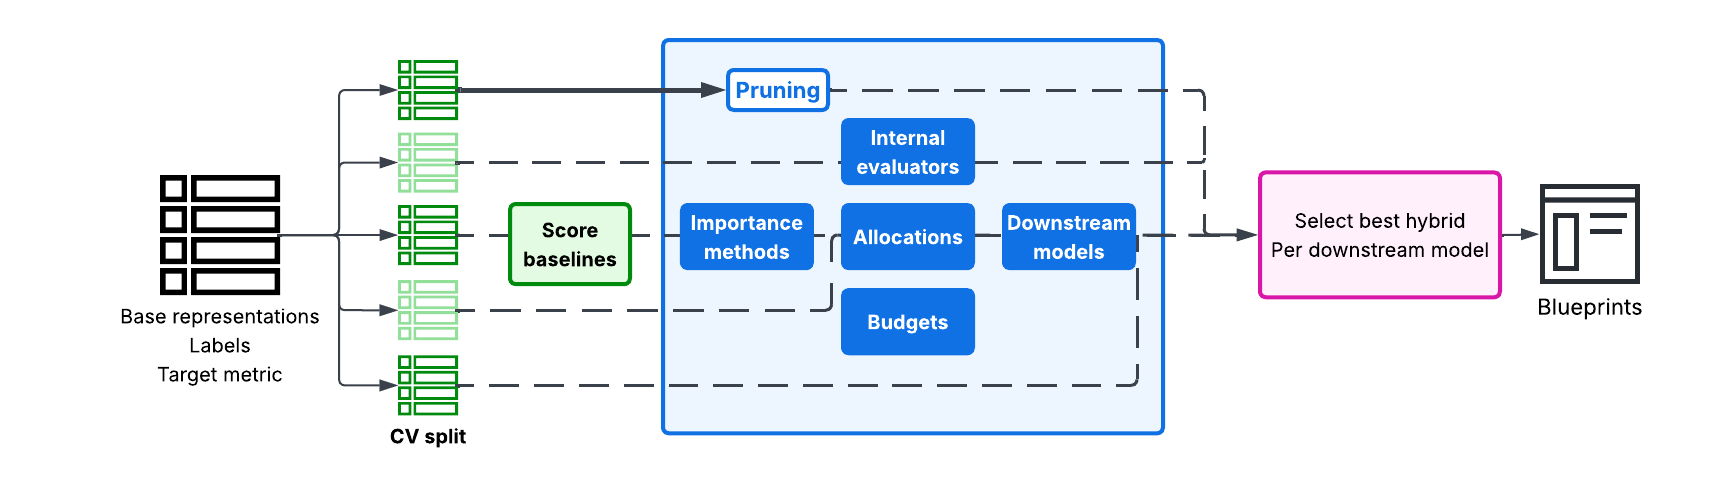
\includegraphics[width=\textwidth,height=0.72\textheight,keepaspectratio]{figures_code_input/hybrid_search_space.png}
    \caption[Schematic overview of the hybrid search.]{Schematic overview of the hybrid search. The inputs (left) are split into five cross-validation folds, and the single representations are scored as baselines. Each fold is searched over importance methods, allocation methods, budgets, internal evaluators and downstream models (center), with adaptive pruning on the first two folds of each search. The best hybrid for each downstream model is stored as a blueprint (right).}
    \label{fig:hybrid_search_space}
\end{figure}
% [TRIM 2026-09-30] paragraph removed, text in cuts file

% CODE INPUT
% [TRIM3 2026-09-30] paragraph removed


\subsection{From Base Representations to a Hybrid}\label{sec:method:build}
% [notes moved to thesis_notes_moved.md]

% [TRIM 2026-09-30] paragraph removed, text in cuts file

% [TRIM3 2026-09-30] simplified
% [TRIM 2026-09-30] shortened
% TODO: REVIEW MODIFICATION
% TODO: review, needs manual review
The search is given $K$ frozen representation matrices $\mathbf{X}^{(k)} \in \mathbb{R}^{n\times d_k}$, $k = 1, \dots, K$, for the same $n$ samples, whose widths $d_k$ range from tens to thousands of features. It also takes a label vector $\mathbf{y}$, one group label per sample for cross-validation (for example its scaffold), the dataset's metric, the task type, one or more downstream models and a list of budgets. It returns a hybrid of at most $B$ features before any augmentation features added outside the budget (Section~\ref{sec:method:augmentation}), where the budget $B$ is a maximum rather than a target, and a blueprint that records the settings needed to rebuild it.

% [TRIM 2026-09-30] paragraph removed, text in cuts file

% [TRIM3 2026-09-30] simplified
% [TRIM2 2026-09-30] LightGBM pre-screen details moved to Additional file app:add:comparator_prescreen; the full-width comparator sentence kept, with its subject restated
% TODO: review, needs manual review
% TODO: REVIEW MODIFICATION
Representations differ in scale, distribution and missingness. Pooling them before splitting would leak validation-set statistics into training, a well-documented source of optimistic bias in feature selection \citep{Ambroise2002, Vabalas2019}, so all preprocessing that uses the labels, and all scaling and imputation, runs within each cross-validation fold; the label-free TCGA reductions are the exception (Section~\ref{sec:method:reps}). When a single representation is scored, missing values are imputed with training-fold medians and entirely missing features are dropped. In the hybrid, missing values are set to 0, and every feature, binary bits included, is standardized with training-fold statistics only. Binary features stay 0/1 only when the search scores a single representation to pick the best single representation that the hybrid is compared with, and representations wider than 5,000 features are pre-screened for that step only (Additional file~\ref{app:add:comparator_prescreen}).

% [TRIM3 2026-09-30] simplified
% [TRIM2 2026-09-30] outer-fold statement reduced to a pointer to 'Splitting rules'; Koenig fold-count example moved to Additional file app:add:fold_counts
% TODO: review, needs manual review
% CODE INPUT
Outer folds follow the splitting rules in Section~\ref{sec:method:datasets}. A representation learned from the labels would be retrained on each outer training fold only; none of the base representations in this chapter is. Within that fold, the search runs its own group-aware cross-validation, 5 folds by default. Inside each of its training folds, a deterministic internal split, the first fold of a 5-fold grouped split, holds out about 20\% of the molecules as whole groups. With fewer than five groups, both splits use as many folds as there are groups (Additional file~\ref{app:add:fold_counts}). Importance and standalone scores come from the training fold only, and the outer test molecules score only the finished hybrid.

% [TRIM3 2026-09-30] simplified
% CODE INPUT
% TODO: review, needs manual review
For each representation $k$, the importance method gives every feature a score $s^{(k)}_j \ge 0$ on the internal training part, which ranks features within that representation only. The standalone score $r_k$ is the internal evaluator's score, fitted on representation $k$ alone, on the internal validation part in the dataset's metric. We rescale $r_k$ to $\tilde r_k$ so that 0 means ``no better than a trivial predictor'', which makes the budget split independent of the metric. For Spearman, Pearson, the Matthews correlation coefficient (MCC) and $R^2$, $\tilde r_k = \max(0, r_k)$. For AUROC and the concordance index, $\tilde r_k = \max(0, 2(r_k - 0.5))$. For RMSE, $\tilde r_k = \max(0, 1 - \mathrm{RMSE}_k/\mathrm{RMSE}_0)$, where $\mathrm{RMSE}_0$ is the error of predicting the training mean, and mean absolute error is rescaled likewise against the training median. For accuracy and weighted F1, $\tilde r_k = \max(0, (r_k - r_0)/(1 - r_0))$, where $r_0$ is the score of always predicting the majority training class.

% [TRIM3 2026-09-30] simplified
% CODE INPUT
% TODO: review, needs manual review
An optional representation count $N$ keeps the $N$ representations with the highest standalone scores on the fold. Each remaining representation receives a weight $w_k = g(\tilde r_k)$, with $g$ set by the allocation method, and a share $b^*_k = B\, w_k / \sum_l w_l$ features, rounded by largest remainder and capped at its width. Thus $\sum_k b_k = \min(B, \sum_k d_k)$ and $b_k \le d_k$, and a representation with $w_k > 0$ keeps at least one feature. The global pool does not use these shares (see below).

% [TRIM3 2026-09-30] simplified
% CODE INPUT
% TODO: review, needs manual review
Let $S_k$ be the top $b_k$ features of representation $k$ by $s^{(k)}_j$, among those with $s^{(k)}_j > 0$; if none scores above 0, its full $b_k$ is taken. The cut exists because tree importance gives exactly 0 to every feature no tree split on, and filling the budget with those would pick them by their position in the matrix. The hybrid is $\mathbf{H} = [\mathbf{X}^{(1)}_{:,S_1}, \dots, \mathbf{X}^{(K)}_{:,S_K}]$, with $\sum_k |S_k| \le B$, so it can be narrower than its budget.

% [TRIM3 2026-09-30] simplified
% CODE INPUT
% TODO: review, needs manual review
A configuration assigns one value to every searched setting. It is scored by fitting the downstream model on the hybrid in each fold of the search and averaging the held-out scores. The winner is picked separately for each pair of downstream model and budget, never across models. Because this score chose among many configurations, it is optimistic \citep{Varma2006, Cawley2010}, so the comparison we report is nested. The whole search runs inside each outer training fold, and the winning settings are rebuilt there and scored once on the untouched outer test fold, both for the winner at each budget and for each downstream model's best across budgets. The inner search score minus the outer test score is \textbf{[RESULT NEEDED: inner minus outer test score, per dataset, in its own metric]}.

% [TRIM3 2026-09-30] simplified
% [TRIM 2026-09-30] shortened
% CODE INPUT
% TODO: review, needs manual review
Chapter~\ref{chap:similarity} uses two variants of this search. Under label noise, training quantities use the noisy labels and held-out scoring uses clean labels unless stated otherwise. Under the nearest-neighbor objective, each molecule's activity is predicted from its five nearest neighbors in the feature space (Chapter~\ref{chap:similarity}, ``Similarity in a hybrid'').

% TODO: Figure 5.1: the search pipeline schematic. Does not exist yet.


\paragraph{Blueprints.}

% [TRIM 2026-09-30] paragraph removed, text in cuts file

% [TRIM3 2026-09-30] simplified
% [TRIM2 2026-09-30] field list cut (Listing lst:blueprint gives it); stored-score sentence changed to match the code, see note under the listing comment
% TODO: review, needs manual review
% TODO: REVIEW MODIFICATION
A blueprint records the search settings needed to rebuild the winning hybrid, so that its features can be examined and the hybrid rebuilt on new datasets. On other molecules, a rebuild re-scores the representations and re-picks the features, so it need not recreate the same hybrid. Some fields serve analysis only, such as which representations fed the hybrid on each fold, and each representation's stored score, measured on every molecule the search saw. A rebuild never splits the budget with this stored score, and the per-fold rebuild in the experiments reads it only to choose representations when the representation count is set and no per-fold scores are given.

% [TRIM3 2026-09-30] simplified
% TODO: REVIEW MODIFICATION -- blueprint shown as a data structure. Every field name and type is copied from the
% Blueprint class in src/kirby/find_best_hybrid.py:1415-1553 (read 2026-09-30). The comments on which fields a rebuild
% reads come from build_fold_hybrid in tests/experiments/_shared.py:5091 (the per-fold rebuild the experiments use).
% That rebuild reads rep_scores in one case (see the comment on that field). The paragraph above says a rebuild never
% reads the stored score; that sentence needs your decision.
% [TRIM2 2026-09-30] stored-score sentence settled against the code (read 2026-09-30): apply_blueprint in src/kirby/find_best_hybrid.py never reads rep_scores;
% [TRIM2 2026-09-30] build_fold_hybrid in tests/experiments/_shared.py:5256-5285 reads it only to rank representations when rep_count is set and no per-fold
% [TRIM2 2026-09-30] scores are passed, and never passes it to create_hybrid for the budget split. The prose above now says this.
% [TRIM2 2026-09-30] step_size field ('Left from a removed method', greedy only) removed from Listing lst:blueprint
% TODO: review, needs manual review
Listing~\ref{lst:blueprint} lists every field of a blueprint and its type.
\begin{lstlisting}[float=htbp, breaklines=true, basicstyle=\scriptsize\ttfamily, columns=fullflexible, keepspaces=true, frame=single, caption={Fields of a blueprint and their types. Comment lines group the fields, and each field is given with its type and, where needed, a comment on its meaning.}, label=lst:blueprint, captionpos=b]
Blueprint
  # What the search chose. A rebuild reads all of these.
  reps                  : list[str]           # every representation searched, not only those used
  rep_count             : int or None         # how many of them may contribute; None = all
  budget                : int                 # most features the hybrid may have
  allocation_method     : str
  importance_method     : str
  internal_evaluator    : str
  objective             : str                 # 'predictive' or 'similarity'

  # How the search scored configurations.
  metric                : str
  lower_is_better       : bool
  task_type             : str                 # 'regression' or 'classification'
  n_folds               : int
  seed                  : int

  # Augmentation settings. A rebuild reads all of these.
  augmentation_strategy : str
  aug_per_source_budget : int, or {source: int}, or None
  augmentation_margin   : float
  augmentation_fraction : float or None
  candidate_ranking     : str
  augmentation_threshold: float or None
  augmentation_budget   : int
  aug_max_candidates    : int

  # Stored for inspection.
  rep_scores            : {representation: float}
                          # each representation's best score over every molecule the search saw;
                          # the rebuild uses it to choose which representations to keep only when
                          # rep_count is set and no per-fold scores are given
  allocation_per_fold   : {fold: {representation: int}}      # features each representation got
  kept_augmentations    : {fold: {source: list[int]}}         # extra features kept, by index
\end{lstlisting}


% [TRIM2 2026-09-30] signed-off original 'The blueprint does not store selected feature indices...' removed; the rewrite below is kept. Text in cuts2 file

% [TRIM3 2026-09-30] simplified
% [TRIM 2026-09-30] shortened
% [TRIM2 2026-09-30] cut 'Re-running the recipe without labels is refused...'
% TODO: REVIEW MODIFICATION
% TODO: review, needs manual review
The blueprint stores how many features each representation received in each fold and which augmentation features were kept, but not the selected base-representation features. It can be reused in two ways. Re-running its settings on new labeled data recomputes importance and standalone scores, so the features adapt but may differ. Alternatively, the exact features of a labeled fit can be taken from new molecules, which needs no labels and so is the only option for unlabeled molecules, but assumes the same features matter. Importance and allocation can also be computed within k-means clusters of the molecules' ECFP fingerprints, to ask whether the budget split changes across chemical space.

% [TRIM2 2026-09-30] signed-off original 'It also provides a registry...' removed; the rewrite 'A separate explanation step...' below is kept. Text in cuts2 file

% [TRIM3 2026-09-30] simplified
% [TRIM 2026-09-30] shortened
% TODO: REVIEW MODIFICATION
% TODO: review, needs manual review
Because the blueprint does not store feature names, a separate explanation step, run on a finished hybrid, records where each selected feature came from and, for some representations, what it means. An ECFP4 bit is named by the atom environment that sets it, written as a SMILES fragment from a molecule with the bit set. MACCS keys are named by their SMILES arbitrary target specification (SMARTS) pattern and a short name, and descriptor features by descriptor name. Protein composition, descriptor and k-mer features, antibody composition, one-hot, BLOSUM, structural and inverse-folding features, gene-expression pathway sets and PCA components are named too. MAP4 and DRFP features get only a bit index, and Avalon, Mordred, atom-pair, graph-kernel and learned-embedding features only the representation name and dimension index.

\subsection{The Search Space}\label{sec:method:searchspace}
% [notes moved to thesis_notes_moved.md]

% [TRIM3 2026-09-30] simplified
% [TRIM 2026-09-30] shortened
% TODO: REVIEW MODIFICATION
% TODO: review, needs manual review
Selecting features raised several questions: how to measure a feature's importance, how many features to take from each representation, and how to score a candidate feature set. As with the choice of representation, different prediction tasks preferred different answers, so the search treats each question as a setting and chooses its value per dataset.

% [TRIM3 2026-09-30] simplified
% CODE INPUT
% TODO: review, needs manual review
Every combination of setting values is built and scored, because the settings interact; for example, the best budget depends on the downstream model, as shown below for nanobody thermostability. The grid measures, rather than assumes, the chapter's claim that no single setting suits every dataset, a claim motivated by, but not proved by, the result that no learning method is best on every problem \citep{Wolpert1996}.

% [TRIM3 2026-09-30] simplified
% CODE INPUT
% [RESTORE 2026-09-30] Ch5b-2
% TODO: review, needs manual review
Six settings are searched, namely the downstream model, the budget, the representation count, the importance method, the allocation method and the internal evaluator. Table~\ref{tab:search_tiers} gives their values at the full and fast tiers, and Additional file~\ref{app:searchspace} the defaults and the number of configurations per downstream model. The importance method is LightGBM gain, TreeSHAP or DeepLIFT. It is searched because importance depends on the model as well as on the data \citep{Dong2020}. The three methods come from different model families and rank features differently, and a different ranking builds a different hybrid. The search objective and augmentation are not searched within a single search; each objective and each augmentation condition is a separate search.

% [TRIM3 2026-09-30] simplified
% [TRIM 2026-09-30] shortened
% CODE INPUT
% TODO: review, needs manual review
The downstream model is trained on the finished hybrid. Five are searched, namely random forest, XGBoost, LightGBM, SVM and a deep neural network (DNN), and a Gaussian process is added on humanness (Section~\ref{sec:method:models}). The downstream model determines which features are useful and how many it can use, so the best hybrid for one model need not be the best for another.

% [TRIM3 2026-09-30] simplified
% CODE INPUT
% TODO: review, needs manual review
The budget is the maximum number of features in the hybrid, and eight budgets are searched (10, 25, 50, 100, 250, 500, 1,000 and 2,000 features). Too few features leave informative ones out, and too many add uninformative ones that give small datasets room to overfit. Budgets above the number of training molecules are kept. In a preliminary 5-fold run on nanobody thermostability, with an earlier budget list that included 300 features, SVM performed best at 300 features (Spearman 0.6384), DNN, LightGBM and random forest at 50, and XGBoost at 100. \textbf{[RESULT NEEDED: best budget per downstream model on nanobody thermostability, full runs]}

% [TRIM3 2026-09-30] simplified
% [TRIM 2026-09-30] shortened
% CODE INPUT
% [RESTORE 2026-09-30] Ch5b-3
% TODO: review, needs manual review
Each dataset has a fixed set of base representations, chosen before the search (Table~\ref{tab:dataset_reps}). The representation count (2, 3, 5 or all) sets how many may contribute features, keeping those with the highest standalone scores on each fold. It is the only step that drops whole representations before allocation, and correlation between representations plays no part in it. It is searched because datasets differ in how many representations are worth using, and pooled feature selection over all representations has no such setting. Every allocation method is paired with every count. In preliminary runs, some datasets performed best with 2 or 3 representations and others with all 10. \textbf{[RESULT NEEDED: datasets best with 2 or 3 representations and with all, full runs]}

\subsubsection{Feature Importance Scoring}
% [notes moved to thesis_notes_moved.md]

% TODO: this is out of date

% What were the qualifications for correlation/filtering allocation strategies? Can I formalize this a bit?
% [TRIM 2026-09-30] paragraph removed, text in cuts file

% [TRIM3 2026-09-30] simplified
% [TRIM 2026-09-30] shortened
% TODO: REVIEW MODIFICATION
% TODO: review, needs manual review
The importance method gives every feature of one representation a single non-negative score, from a model freshly fitted on that representation alone; the downstream model is not used. Only the order within a representation is used, so scores are not normalized. Split-based tree importance is biased toward features with many possible split points \citep{Strobl2007}, which matters here because binary fingerprint bits sit beside continuous embeddings.

% [TRIM3 2026-09-30] simplified
% [TRIM 2026-09-30] shortened
% [TRIM2 2026-09-30] pointer to Additional file app:add:design_experiments added; the preliminary comparisons below moved there
% TODO: REVIEW MODIFICATION
% TODO: review, needs manual review
No single importance method worked best across datasets and downstream models, and the preferred method changed with the dataset. We kept three methods whose rankings did not correlate strongly with each other and whose selected features performed well as model input (Additional file~\ref{app:add:design_experiments}).

% TODO: background on each of these, also how do I name these in text
% [TRIM 2026-09-30] paragraph removed, text in cuts file

% [TRIM3 2026-09-30] simplified
% [TRIM 2026-09-30] shortened
% TODO: REVIEW MODIFICATION
% TODO: review, needs manual review
We score features using LightGBM gain importance, SHapley Additive exPlanations (SHAP) values for tree ensembles (TreeSHAP) and DeepLIFT (Deep Learning Important FeaTures) \citep{Shrikumar2017}. LightGBM gain measures how much a feature reduced the training loss where trees split on it \citep{ke2017lightgbm}. TreeSHAP gives each feature's exact Shapley value for each molecule's prediction from a tree model \citep{Lundberg2020}. DeepLIFT measures how much a feature moves the output of a small network, trained with Adam \citep{Kingma2015}, away from its output on an all-zero reference input, which after standardization places every feature at its training mean \citep{Shrikumar2017, Kokhlikyan2020, Ancona2018}. On Caco-2, the median share of features scoring above 0 was 30\% for LightGBM gain, 70\% for TreeSHAP and 90\% for DeepLIFT (preliminary, over 10 representations and 3 folds). Table~\ref{tab:importance_methods} gives the settings of each method, including the pre-screen of representations wider than 2,000 features.

% CODE INPUT
\begin{table}[htbp]
\centering
\small
\begin{adjustbox}{max width=\textwidth,max totalheight=0.78\textheight}
\begin{tabular}{@{}P{0.15\linewidth}P{0.24\linewidth}P{0.22\linewidth}P{0.17\linewidth}P{0.16\linewidth}@{}}
\toprule
Method (family) & Model fitted per representation & Score of one feature & Classification labels & Representations over 2{,}000 features \\
\midrule
LightGBM gain (split gain) & LightGBM, 50 trees, maximum depth 6 & Loss reduction of every split on the feature, summed over all trees; 0 if never split on & One model on the class labels & Only the 2{,}000 highest-variance features are fitted; the rest score 0 \\
TreeSHAP (Shapley values) & Random forest, 50 trees, maximum depth 10 & Mean absolute Shapley value over the training molecules & Binary: positive class. Multiclass: mean absolute value over classes & As for LightGBM gain \\
DeepLIFT (reference-based attribution) & Small neural network, ReLU hidden layers of 64 and 32 units, 100 full-batch epochs of Adam, learning rate 0.001 & Mean absolute attribution against an all-zero reference, Rescale rule & Binary: positive class. Multiclass: mean absolute value over classes & Every feature is scored \\
\bottomrule
\end{tabular}
\end{adjustbox}
\caption[Settings of the three importance methods searched.]{Settings of the three importance methods. Each method is fitted separately on every representation inside each fold, and settings not listed are the library defaults.}
\label{tab:importance_methods}
\end{table}

% [TRIM2 2026-09-30] signed-off original 'When searching for the features... thse...' removed; the rewrite below is kept. Text in cuts2 file

% [TRIM3 2026-09-30] simplified
% [TRIM 2026-09-30] shortened
% TODO: REVIEW MODIFICATION
% TODO: review, needs manual review
The full search sweeps all three importance methods, whereas the fast tier uses LightGBM gain only (Table~\ref{tab:search_tiers}).

% [TRIM2 2026-09-30] four preliminary comparisons of importance methods and Table tab:importance_wins moved verbatim to Additional file app:add:design_experiments


\subsubsection{Feature Allocation Methods}\label{sec:method:allocation}
% [notes moved to thesis_notes_moved.md]

% TODO: allocation strategies completely out of date
% Check framework doc?
% [TRIM 2026-09-30] paragraph removed, text in cuts file

% [TRIM3 2026-09-30] simplified
% TODO: REVIEW MODIFICATION
% TODO: review, needs manual review
The allocation method decides how many of the $B$ features each representation contributes; the importance method decides which. Of the five methods searched, four give each representation a fixed share computed from its rescaled standalone score (linear, squared, softmax and rank-decay allocation). The fifth, the global pool, lets the candidate features offered by every representation compete in one importance ranking.

% TODO: completely replace this is SO out of date, I need a version of this for all the allocation strategies I'm using, as well as the knobs

% \begin{enumerate}
%     \item \textbf{Split:} Divide training data into allocation-train (80\%) and validation (20\%) subsets using scaffold splitting.

%     \item \textbf{Initialize:} Set current feature set to empty, remaining budget to $B$.

%     \item \textbf{Rank features:} For each representation $r \in \{base_1, base_2, \dots base_m\}$, train RFs using the base representations individually, then rank features by mean decrease in impurity.

%     \item \textbf{Iterate:} While remaining budget $\geq$ step\_size and patience not exhausted:
%     \begin{enumerate}
%         \item For each representation, try adding the top step\_size candidates from its ordered list to the current feature set.
%         \item Train a RF using the tentative feature set.
%         \item Evaluate $R^2$ on the validation set.
%         \item Select the representation whose addition yields the highest validation $R^2$.
%         \item Permanently add step\_size features from the winning representation; remove from its candidate list.
%         \item If validation $R^2$ does not improve for patience consecutive rounds, terminate early.
%     \end{enumerate}

%     \item Re-compute importance scores for the features of the new hybrid on the full training data. For each representation, select the top $n_r$ features according to the allocation determined above, where $n_r$ is the number of features allocated to representation $r$ during iteration.
% \end{enumerate}

% This greedy approach works better on larger datasets, as the size of the validation set may not be enough to gain meaningful insights from.

% TODO: this is not what's happening
% [TRIM 2026-09-30] paragraph removed, text in cuts file

% [TRIM3 2026-09-30] simplified
% TODO: REVIEW MODIFICATION
% TODO: review, needs manual review
The four fixed-share methods compute shares from the standalone score on the internal validation part. Only linear allocation makes the share proportional to that score. All four assume that representations with stronger predictive performance contribute more valuable features.

% [TRIM 2026-09-30] paragraph removed, text in cuts file

% [TRIM 2026-09-30] shortened
% TODO: REVIEW MODIFICATION
% [TRIM3 2026-09-30] paragraph removed

% [TRIM 2026-09-30] paragraph removed, text in cuts file

% [TRIM3 2026-09-30] simplified
% TODO: REVIEW MODIFICATION
% TODO: review, needs manual review
The assumption fails when a strong representation owes its score to a few features, so that a large share fills with weak ones. Fixed shares also ignore complementarity, so two representations carrying the same information both receive a share. Only the global pool ranks features from different representations against each other.

% TODO: explain why the greedy approach was tried, but it's too computationally intensive and actually quite ineffective
% TODO: explain framework experiments and how they helped here

% [TRIM3 2026-09-30] simplified
% CODE INPUT
% TODO: review, needs manual review
The fixed-share methods differ only in how $w_k$ is computed from $\tilde r_k$ (Table~\ref{tab:alloc_methods}), with settings fixed for every dataset. Under linear and squared allocation, a representation with rescaled score 0 receives 0 features. Under softmax and rank decay, no representation receives 0 features because of its score. Since every rescaled score lies between 0 and 1, softmax cannot give one representation most of the budget, and with 10 representations the best takes at most 23.2\% of it. Rank decay uses only the order, so with 10 representations the best receives 27.3\% and the tenth 1.8\%, whatever the gaps between their scores. Table~\ref{tab:alloc_example} gives a worked example.

% CODE INPUT
\begin{table}[htbp]
\centering
\small
\begin{adjustbox}{max width=\textwidth,max totalheight=0.78\textheight}
\begin{tabular}{@{}P{0.13\linewidth}P{0.24\linewidth}P{0.14\linewidth}P{0.24\linewidth}P{0.19\linewidth}@{}}
\toprule
Method & Weight $w_k$ & Fixed setting & How features are chosen & When a representation receives 0 features \\
\midrule
Linear & $\tilde r_k$ & none & Top $b_k$ of its own ranking & $\tilde r_k = 0$ \\
Squared & $\tilde r_k^{\,2}$ & power 2 & Top $b_k$ of its own ranking & $\tilde r_k = 0$ \\
Softmax & $\exp\big((\tilde r_k - \max_l \tilde r_l)/T\big)$ & $T = 1$ & Top $b_k$ of its own ranking & never from its score \\
Rank decay & $e^{-0.3\rho_k}$, $\rho_k$ = rank by score, 0 for the best & decay 0.3 & Top $b_k$ of its own ranking & never from its score \\
Global pool & $\tilde r_k^{\,2}$, sizing its offer to a pool of $2B$ candidates & power 2; pool $2B$ & Top $B$ of one joint ranking over all offered candidates & $\tilde r_k = 0$, or none of its candidates in the joint top $B$ \\
\bottomrule
\end{tabular}
\end{adjustbox}
\caption[The five allocation methods searched.]{The five allocation methods. $w_k$ is the weight computed from representation $k$'s rescaled standalone score $\tilde r_k$, $B$ is the budget, $b_k$ is the share of representation $k$, $\rho_k$ is its rank by score and $T$ is the softmax temperature. Under every method, a representation left out by the representation count, or whose standalone fit fails, receives no features.}
\label{tab:alloc_methods}
\end{table}

% CODE INPUT
\begin{table}[htbp]
\centering
\begin{adjustbox}{max width=\textwidth,max totalheight=0.78\textheight}
\begin{tabular}{@{}lccc@{}}
\toprule
Method & $\tilde r_1 = 0.6$ & $\tilde r_2 = 0.5$ & $\tilde r_3 = 0.2$ \\
\midrule
Linear & 46 & 39 & 15 \\
Squared & 55 & 39 & 6 \\
Softmax & 39 & 35 & 26 \\
Rank decay & 44 & 32 & 24 \\
\bottomrule
\end{tabular}
\end{adjustbox}
\caption[Worked example of the four fixed-share allocation methods.]{Worked example of the four fixed-share allocation methods for a budget of 100 features and three representations. Each entry is the number of features a representation receives, with shares rounded by largest remainder.}
\label{tab:alloc_example}
\end{table}

% [TRIM3 2026-09-30] simplified
% CODE INPUT
% TODO: review, needs manual review
The global pool sizes each representation's offer with squared weights $\tilde r_k^{\,2}$, as shares of a pool of $2B$ candidate features, each offer capped at the representation's width and holding only features scoring above 0. The same importance method is fitted once on the joined offers, and the hybrid keeps the top $B$ features that score above 0. Each representation's count is therefore an outcome of the joint ranking, with no minimum of one feature, and a feature's rank depends on what the other representations offered. The cost is one extra importance fit per configuration.

% [TRIM 2026-09-30] paragraph removed, text in cuts file

% [TRIM3 2026-09-30] simplified
% [TRIM2 2026-09-30] greedy paragraph and the allocation comparison moved verbatim to Additional file app:add:design_experiments; first sentence kept with a pointer
% CODE INPUT
% TODO: review, needs manual review
The five methods were chosen in a preliminary comparison (Additional file~\ref{app:add:design_experiments}).

\subsubsection{Search Configuration and Internal Evaluation}
% [notes moved to thesis_notes_moved.md]

% [TRIM 2026-09-30] paragraph removed, text in cuts file

% [TRIM3 2026-09-30] simplified
% TODO: REVIEW MODIFICATION
% TODO: review, needs manual review
Features that help a random forest may not help an SVM, and vice versa, because variable importance depends on the model \citep{Dong2020}. The internal evaluator is a model fitted on one representation at a time, separate from the downstream model. Four are searched, namely random forest, DNN, LightGBM and the matched evaluator, a model of the downstream model's own family, and none is chosen in advance. Each is fitted on the internal training part and scored on the internal validation part in the dataset's metric.

% [TRIM 2026-09-30] paragraph removed, text in cuts file

% [TRIM3 2026-09-30] simplified
% TODO: REVIEW MODIFICATION
% TODO: review, needs manual review
The internal evaluator's scores set how the budget is split and which representations are kept; it does not rank features within a representation. Judging a feature set by the score of a model fitted on it is the wrapper idea of \citet{Kohavi1997}.

% TODO: need additional files to specify architectures

% TODO: does match always work? custom downstream model?

% TODO: these numbers are outdated
% [TRIM 2026-09-30] paragraph removed, text in cuts file

% [TRIM3 2026-09-30] simplified
% [TRIM 2026-09-30] shortened
% TODO: REVIEW MODIFICATION
% TODO: review, needs manual review
The full search tests every combination of the six settings under 5-fold cross-validation, giving 8,160 configurations per dataset where all five downstream models run, fewer where one is left out, and 10,080 on humanness, where a Gaussian process is added. A fast-tier search has 816. Additional file~\ref{app:add:search_size} gives the breakdown by downstream model and the number of model fits.

% TODO: mention representation knobs

% [TRIM 2026-09-30] paragraph removed, text in cuts file

% [TRIM3 2026-09-30] simplified
% [TRIM 2026-09-30] shortened
% TODO: REVIEW MODIFICATION
% TODO: review, needs manual review
Importance scores are computed once per fold and importance method, and standalone scores once per fold and internal evaluator. Every configuration reuses them, so the cost grows more slowly than the number of configurations.

% TODO: REVIEW MODIFICATION -- rewritten; the original paragraph is commented out below.
% When I began to implement this idea, I figured that there would be a fairly straightforward way to select the most informative features. However, I began to ask some questions. How do you measure feature importance? If you're starting with a handful of input representations, how many features do you take from each? How do you score these potential feature sets?  Unfortunately, my one-size-fits-all hypothesis rang true on multiple fronts. As I found out, different prediction tasks prefer different answers to all of those questions. So to figure out how to even go about selecting the best features, I realized I had to sweep a search space.
% [TRIM 2026-09-30] paragraph removed, text in cuts file

% TODO: explain framework experiments
% [TRIM 2026-09-30] paragraph removed, text in cuts file

% [TRIM3 2026-09-30] simplified
% [TRIM2 2026-09-30] moved verbatim to Additional file app:add:design_experiments; first sentence kept with a pointer
% TODO: REVIEW MODIFICATION
% TODO: review, needs manual review
Preliminary design experiments set the values each setting may take (Additional file~\ref{app:add:design_experiments}).

% [TRIM3 2026-09-30] simplified
% [TRIM 2026-09-30] shortened
% CODE INPUT
% TODO: review, needs manual review
For random forest, LightGBM and DNN downstream models, the matched evaluator is already among the four, so these are searched with 3 evaluators. For XGBoost and SVM, and for the Gaussian process on humanness, it adds an evaluator of that family, giving 4. Only the DNN evaluator shares its downstream model's architecture and training settings, and even it draws its 20\% early-stopping molecules at random, whereas the downstream DNN splits them by the outer split's groups. Additional file~\ref{app:add:model_settings} gives every evaluator setting.

% [TRIM2 2026-09-30] user-supplied downstream model paragraph cut; one sentence now in Limitations

% [TRIM2 2026-09-30] matched-evaluator preliminary comparison moved verbatim to Additional file app:add:design_experiments


\subsection{Augmentation}\label{sec:method:augmentation}
% [notes moved to thesis_notes_moved.md]

% TODO: review, also I think this is out of date
% [TRIM 2026-09-30] paragraph removed, text in cuts file

% [TRIM3 2026-09-30] simplified
% [TRIM 2026-09-30] shortened
% TODO: REVIEW MODIFICATION
% TODO: review, needs manual review
Some feature sets are too small or too specialized to take part in budget allocation, such as MACCS fingerprints (167 features) or log-likelihood ratios (3 features). Others, such as mutation features that record differences from a parent antibody, carry meaning only beside a full representation. Excluding them would lose potentially useful signal, but including them would distort the budget split, since they cannot contribute many features. We therefore add them as augmentation, calling the finished hybrid $\mathbf{H}$ the base and the feature sets that supply extra features the donors.

% TODO: I need a better list to describe augmentations
% [TRIM 2026-09-30] paragraph removed, text in cuts file

% [TRIM3 2026-09-30] simplified
% [TRIM 2026-09-30] shortened
% TODO: REVIEW MODIFICATION
% TODO: review, needs manual review
Donors are set per dataset (Augmentation column of Table~\ref{tab:dataset_reps}). They range from small fingerprints such as MACCS to structural sets such as 3D pharmacophores and Coulomb matrix eigenvalues, and include features that describe only differences between variants, such as antibody mutation features. MACCS is a donor on four of the six small-molecule datasets and a base representation on MDR1--MDCK efflux. On QM9, MACCS is not offered and the topological torsion fingerprint (2,048 features) is a donor, the only wide one. \citet{Bahia2023} found that combining 2D and 3D descriptors gave many more significant models across six protein--ligand series (461 structures), which they attribute to complementary properties. Their 3D descriptors came from bioactive conformations in the Protein Data Bank, whereas our 3D donors use one generated conformer per molecule.
% TODO: add augmentation subsection

% [TRIM3 2026-09-30] simplified
% CODE INPUT
% TODO: review, needs manual review
Donor features are ranked by what the base gets wrong. Inside each outer training fold, an 80/20 internal split keeps each scaffold or sequence group on one side. A small random forest (50 trees, depth at most 10) is fitted on the base features, and 3-fold group-aware cross-validation gives out-of-fold residuals $r_i = y_i - \hat{y}^{\mathrm{oof}}_i$ for the internal-training molecules, where for binary tasks $\hat{y}$ is the positive-class probability. In-sample residuals would shrink toward zero. All donor features are pooled, each is scored by its absolute Pearson correlation with the residuals, $c_j = |\rho_{\mathrm{P}}(\mathbf{x}_j, \mathbf{r})|$, and the top $M = 50$ go forward. Ranking against $\mathbf{y}$ would favor features that repeat what the base captures; ranking against $\mathbf{r}$ favors features that explain its errors, as in gradient boosting \citep{friedman2001greedy} and least angle regression \citep{efron2004lars}.

% [TRIM3 2026-09-30] simplified
% CODE INPUT
% TODO: review, needs manual review
Blocks of the top $k \in \{0, 5, 10, 20, 40\}$ ranked features, capped at the number of candidates, are each added to the base and scored with the downstream model on the internal-validation molecules. The chosen $k^*$ has the best score and must beat $k=0$, which wins ties, so keeping no extras is the default. Five block choices instead of about 50 accept-or-reject decisions leave less room to overfit a small validation set \citep{Cawley2010}. The chosen donors and feature positions are stored and re-extracted for the outer fold. \textbf{[RESULT NEEDED: how often $k^*=0$, and per-fold scores for no, uncapped and capped augmentation, per dataset and downstream model]}

% [TRIM3 2026-09-30] simplified
% CODE INPUT
% TODO: review, needs manual review
In uncapped mode, extras are appended outside the budget, so the final width is $|\mathbf{H}| + k^*$, at most $B + 40$ features. In capped mode, they displace base features and the width stays at most $B$. The base features are ranked once by random forest importance (50 trees, depth at most 10) and the $k^*$ weakest are dropped, after any unspent budget is filled, keeping at least one base feature. Uncapped augmentation and no augmentation differ in width at the same $B$, so their comparison mixes better features with more features. Capped mode, where an extra must beat a base feature, removes this difference.

% [TRIM3 2026-09-30] simplified
% [TRIM 2026-09-30] shortened
% CODE INPUT
% [RESTORE 2026-09-30] Ch5b-6
% TODO: review, needs manual review
Augmentation is a separate condition rather than a searched setting, so each dataset with donors is searched three times, with no, uncapped and capped augmentation. Fourteen of the 16 datasets run all three, while humanness and trastuzumab--HER2 binding have no donors. The three conditions also run under the nearest-neighbor objective, on the datasets given in Chapter~\ref{chap:similarity}, ``Similarity in a hybrid''. In a second use, a user keeps one strong representation at full width as the base and adds a few extras, with $B$ its width, so only uncapped mode makes sense. We test this use, with planted decoy features, in Section~\ref{sec:method:comparators}. This use matters for adoption, because a chemist can keep the representation they already trust and learn which few outside features help, and how many. Augmentation also asks directly whether another representation holds signal the base lacks (Chapter~\ref{chap:flaws}). On Koenig expression, the mutation features and the ESM-2 log-likelihood ratios reach the model only through augmentation. \textbf{[RESULT NEEDED: donors kept most often, per domain]}

% [TRIM3 2026-09-30] simplified
% CODE INPUT
% TODO: review, needs manual review
The residual ranking has four limitations. $|\rho_{\mathrm{P}}|$ captures only linear relations, one feature at a time. It ignores redundancy, so two near-identical donor features can both rank high. Donors are pooled with no per-donor limit, so a 2,048-feature donor gets more chances than a 49-feature one. Finally, the margin over $k=0$ is zero, so a near-tie on one internal split can admit extras.

% [TRIM3 2026-09-30] simplified
% CODE INPUT
% TODO: review, needs manual review
Table~\ref{tab:aug_conditions} summarizes the three conditions.

% CODE INPUT
\begin{table}[htbp]
\centering
\small
\begin{adjustbox}{max width=\textwidth,max totalheight=0.78\textheight}
\begin{tabular}{@{}P{2.4cm}P{3.0cm}P{4.6cm}P{3.6cm}@{}}
\toprule
Condition & Final width (features) & What an extra feature must beat & Datasets that run it \\
\midrule
No augmentation & at most $B$ & nothing is offered & all 16 \\
Uncapped & $|\mathbf{H}| + k^*$, at most $B + 40$ & keeping no extras & the 14 with donors \\
Capped & at most $B$ & keeping no extras, and the weakest base feature it replaces & the 14 with donors \\
\bottomrule
\end{tabular}
\end{adjustbox}
\caption[The three augmentation conditions.]{The three augmentation conditions. $B$ is the budget and $|\mathbf{H}|$ the width of the base hybrid, both in features, and $k^*$ is the chosen number of extra features, which are drawn from a small or specialized feature set offered to the hybrid.}
\label{tab:aug_conditions}
\end{table}


\subsection{Fast Tier and Adaptive Pruning}
% [notes moved to thesis_notes_moved.md]

% [TRIM3 2026-09-30] simplified
% CODE INPUT
% TODO: review, needs manual review
The search can be made cheaper in two ways. The fast tier uses shorter value lists for some settings, fixed in advance and identical on every fast-tier dataset, and accepts a possibly worse answer for a much smaller grid. Adaptive pruning decides during the search from the dataset's own fold scores, and aims to find the same best configuration while no longer scoring configurations that have clearly lost. Without either, the full search does not finish on the largest datasets.

% [TRIM3 2026-09-30] simplified
% CODE INPUT
% TODO: review, needs manual review -- needs your numbers. Four 12-hour jobs are 48 hours, but the old text said "about 40 hours", and TATA promoter (39 h, 5,274 sequences) meets neither criterion as stated. Trastuzumab--HER2 binding (5,000 variants) has no run time given. The code rationale (tests/experiments/dataset_policy.py:658-663, read 2026-09-30) gives the same estimates and does not explain either dataset. LogD is 62 h here but 79 h unpruned in the pruning calibration below; say what differs between the two estimates. Re-checked 2026-09-30: the comment in tests/experiments/dataset_policy.py lists tz_her2_binary at 5,000 rows and nt_promoter_tata at ~39 h under 'past what four 12-hour links can reach ... or past 10,000 rows', which neither meets; the code gives no other criterion. Not changed.
Six of the 16 datasets use the fast tier, namely QM9, LogD, Koenig expression, trastuzumab--HER2 binding, H3K4me3 and TATA promoter (marked in Table~\ref{tab:dataset_reps}). A dataset uses it when the full search would take longer than four consecutive 12-hour jobs can cover, or when it has more than 10,000 molecules or sequences. Estimated full-search run times were about 103 hours for QM9, 64 for Koenig expression, 62 for LogD and 39 for TATA promoter, and H3K4me3 has 18,244 sequences. The values the fast tier drops are still searched on every other dataset, so it is a compromise on compute, not a claim that those values are useless.

% [TRIM2 2026-09-30] moved verbatim to Additional file app:add:design_experiments; first sentence kept with a pointer
% CODE INPUT
The fast lists were chosen by one rule in a preliminary comparison (Additional file~\ref{app:add:design_experiments}).

\subsubsection{Search Tier Settings}
% [notes moved to thesis_notes_moved.md]

% [TRIM3 2026-09-30] simplified
% TODO: review, needs manual review
Table~\ref{tab:search_tiers} gives the values of each setting at both tiers.

% TODO: review, needs manual review
\begin{table}[htbp]
\centering
\begin{adjustbox}{max width=\textwidth,max totalheight=0.78\textheight}
\begin{tabular}{@{}P{0.22\linewidth}P{0.40\linewidth}P{0.30\linewidth}@{}}
\toprule
Setting & Full tier & Fast tier \\
\midrule
Downstream models & Random forest, XGBoost, LightGBM, SVM$^{a}$, DNN; Gaussian process$^{b}$ & Random forest, XGBoost, LightGBM, SVM$^{a}$, DNN \\
Internal evaluators & Matched evaluator, random forest, LightGBM, DNN & Same as full \\
Feature budgets (features) & 10, 25, 50, 100, 250, 500, 1{,}000, 2{,}000 & Same as full \\
Allocation methods & Linear, squared, softmax, rank decay, global pool & Linear, squared, rank decay \\
Importance methods & LightGBM gain, DeepLIFT, TreeSHAP & LightGBM gain \\
Representation counts & 2, 3, 5, all representations & 3, all representations \\
\bottomrule
\end{tabular}
\end{adjustbox}

\smallskip
{\footnotesize $^{a}$SVM is not fitted above 10{,}000 molecules (5{,}000 when augmentation features are added outside the budget). $^{b}$Humanness only. The other two datasets under 1{,}000 samples, nanobody thermostability and PAM50 subtype, drop it for run time.}
\caption[Values searched for each setting at the two search tiers.]{Values searched for each setting at the full and fast tiers. Configurations removed by adaptive pruning are scored on only the first two of the five folds. The matched evaluator belongs to the same model family as the downstream model.}
\label{tab:search_tiers}
\end{table}

\subsubsection{Adaptive Pruning}
% [notes moved to thesis_notes_moved.md]

% [TRIM 2026-09-30] paragraph removed, text in cuts file

% [TRIM3 2026-09-30] simplified
% TODO: REVIEW MODIFICATION
% TODO: review, needs manual review
In adaptive pruning, every configuration is first scored on the first two folds and ranked by its mean over them, in the dataset's own metric. Budgets are scored from smallest to largest. Once every budget up to 100 features is scored, a checkpoint runs within each group of configurations that share a downstream model, internal evaluator and representation count. Pairs of allocation and importance method with no configuration in the group's better half are not searched at larger budgets, although at least one pair per group is kept. Each setting is then voted on within groups that fix every other setting, budget included. The best few values in each group receive a point, and a value is removed if it receives a point in fewer than a cut-off share of groups (Table~\ref{tab:pruning_rules}), but a vote never removes every value. The survivors are scored on the remaining folds, and the best is picked by its mean over all five folds, as without pruning.

% [TRIM3 2026-09-30] simplified
% CODE INPUT
% TODO: review, needs manual review
Configurations far behind after two folds would only confirm their loss on the other three, so pruning stops scoring them. Its one criterion is never to remove a configuration that would have been the best; time saved is secondary. As submitted, every dataset's search uses pruning, at both tiers, and on fast-tier datasets the importance vote does not run because only one importance method is searched. Successive halving \citep{Jamieson2016} and Hyperband \citep{Li2018Hyperband} likewise drop hyperparameter configurations on partial evaluations, here two of the five folds.

% CODE INPUT
% [TRIM3 2026-09-30] paragraph removed

% CODE INPUT
\begin{table}[htbp]
\centering
\small
\begin{adjustbox}{max width=\textwidth,max totalheight=0.78\textheight}
\begin{tabular}{@{}P{2.2cm}P{3.4cm}P{2.8cm}P{1.6cm}P{3.6cm}@{}}
\toprule
Rule & How groups are formed & Kept, or receives a point & Cut-off & Removed on the calibration datasets \\
\midrule
Checkpoint at 100 features & configurations at budgets up to 100 features with the same downstream model, internal evaluator and representation count & (allocation, importance) pairs with a configuration in the better half of the group & better half of the configurations & configurations within groups only; never a whole allocation or importance method \\
\addlinespace
Representation count & every other setting fixed, budget included & best 1 & 10\% of groups & the count of 5 on LogD; the count of 2 on breast cancer PAM50 subtype \\
\addlinespace
Allocation method & every other setting fixed, budget included & best 2 & 20\% of groups & softmax on LogD \\
\addlinespace
Importance method & every other setting fixed, budget included & best 2 & 20\% of groups & DeepLIFT on nanobody thermostability and hERG $K_i$; TreeSHAP on LogD \\
\addlinespace
Internal evaluator & every other setting fixed, budget included & best 3 & 10\% of groups & the matched evaluator of the SVM downstream model on LogD \\
\bottomrule
\end{tabular}
\end{adjustbox}
\caption[The adaptive pruning rules.]{The adaptive pruning rules. Every rule ranks configurations by their mean score over folds 1 and 2 in the dataset's own metric, and the last column gives what the rule removed on the five calibration datasets in a preliminary run.}
\label{tab:pruning_rules}
\end{table}

% [TRIM3 2026-09-30] simplified
% CODE INPUT
% TODO: review, needs manual review
Because votes are grouped by every other setting, a value that is best for a random forest at 25 features is not removed for losing to a DNN at 500 features. One fold is not enough. In the representation-count vote on breast cancer PAM50 subtype after fold 1 alone, 726 of 1,020 groups had every value at an identical score, and ties broken by list order then remove values by accident. After one fold, no cut-off of any vote was safe on the calibration datasets, whereas after two folds each vote had at least one safe cut-off.

% [TRIM3 2026-09-30] simplified
% [TRIM 2026-09-30] shortened
% CODE INPUT
% TODO: review, needs manual review -- calibration budget list taken from tests/experiments/framework/F33_PRUNING_PROCEDURE.md, Step 1 (a procedure document, read 2026-09-30); check it is what the calibration run used.
The cut-offs were calibrated in a preliminary study on five datasets, LogD, hERG $K_i$, breast cancer PAM50 subtype, nanobody thermostability and humanness, by replaying each rule on fold scores from an unpruned five-fold run. A cut-off counts as safe if the best five-fold score is unchanged for each of the 25 combinations of the five downstream models and the five budgets of the calibration run (25, 50, 100, 150 and 300 features), on every dataset. Among safe cut-offs that made the same cuts, we chose the one whose neighboring cut-off was also safe. TreeSHAP accounts for 71\% of LogD's fitting time and was never the best there, so most of the saving comes from it. Estimated run times for eight budgets, without and with pruning, were 79 and 44 hours on LogD, 42 and 35 on hERG $K_i$, 42 and 30 on PAM50 subtype, 32 and 24 on nanobody thermostability, and 15 and 13 on humanness. The calibration applied the votes one after another, whereas the search applies all four at once to the fold 1 and 2 scores. Five datasets form a small calibration set, which limits the rules.

% [TRIM3 2026-09-30] simplified
% CODE INPUT
% TODO: review, needs manual review
% DECISION FOR ADELAIDE: (c) whether one or two voting folds are left out (see the Chapter 5 noise-robustness paragraph, which leaves out one). Text below still says both.
With pruning on, folds 1 and 2 of the search both select the survivors and score them, so the winner's five-fold mean over the search folds is slightly optimistic \citep{Cawley2010}. In the nested comparison these are inner folds, and the outer test fold on which the hybrid and the single representation are compared is untouched. Some experiments instead search over all molecules and compare the hybrid with the single representation on the search's own folds, as in leave-one-fold-out reselection, and there folds 1 and 2 are outer folds. Single representations are never pruned, so a fair comparison in those experiments leaves both voting folds out of both scores, or re-scores without them.

\section{Methods: Experimental Setup}
% [notes moved to thesis_notes_moved.md]
% CODE INPUT
% [TRIM3 2026-09-30] paragraph removed

% [TRIM2 2026-09-30] outer-fold statement reduced to a pointer to 'Datasets and splitting'
% [TRIM3 2026-09-30] simplified
% TODO: review, needs manual review
% CODE INPUT
Every experiment splits each dataset into outer folds as set out in Section~\ref{sec:method:datasets}, except one preliminary analysis of Koenig expression, which uses three outer folds of unequal size. The search sees only the training samples of each outer fold, and the selected features are rebuilt on them and applied unchanged to the held-out samples.

% [TRIM 2026-09-30] shortened
% [TRIM3 2026-09-30] simplified
% CODE INPUT
% [RESTORE 2026-09-30] Ch5c-1 Ch5c-2 Ch5c-3
% TODO: review, needs manual review
The hybrid is compared with the best single base representation at its full number of features, which is what a user would otherwise run. This comparator is chosen per downstream model and per fold from the search's scores on the outer training samples, then refit on those samples and scored on the same held-out samples as the hybrid, so it can differ between folds. Choosing it on the held-out samples would give it an advantage that the hybrid does not get. The hybrid is held to its budget, plus any augmentation features, so the comparator is often many times wider, and both widths are recorded for every fold, since a difference between the two scores is partly a difference in width as well as in method. The main quantity per fold is the hybrid's score minus that of the best single representation, signed so that a positive value means the hybrid scored better (for RMSE the sign is flipped).

% CODE INPUT
Chapter~\ref{chap:similarity} reuses this protocol with noise added to the training labels of each outer fold, while the held-out labels stay clean.


\subsection{Datasets and Splitting}\label{sec:method:datasets}
% [notes moved to thesis_notes_moved.md]

% [TRIM3 2026-09-30] simplified
% TODO: review, needs manual review
The hybrid experiments use 16 datasets from six domains (Table~\ref{tab:datasets}), whose curation is given in Additional file~\ref{app:datasets} and whose representations are listed in Table~\ref{tab:dataset_reps}. Folds keep each group whole, with groups chosen to match what an unseen sample means in each field.

% [TRIM 2026-09-30] paragraph removed, text in cuts file
% TODO: REVIEW MODIFICATION
% [TRIM3 2026-09-30] paragraph removed

% [TRIM2 2026-09-30] both 'No random splits are used...' and 'No split is random...' removed; the reason sentence (Yang2019, Wallach2018) moved into 'Splitting rules'

% [TRIM2 2026-09-30] Table tab:datasets (same 16 rows) deleted; this table relabeled from tab:datasets_modified to tab:datasets
% TODO: REVIEW MODIFICATION
\begin{table}[htbp]
\centering
\footnotesize
\setlength{\tabcolsep}{3pt}
\begin{adjustbox}{max width=\textwidth,max totalheight=0.78\textheight}
\begin{tabular}{P{2.6cm}P{2.5cm}P{2.0cm}P{1.0cm}P{2.4cm}P{2.4cm}}
\toprule
Dataset & Label (unit) & Task, metric & $n$ & Folds grouped by (groups) & Best single representation (score) \\
\midrule
\multicolumn{6}{l}{\textit{Small molecules: ADME and toxicity}} \\
hERG $K_i$ \citep{Zdrazil2023} & p$K_i$ & regression, RMSE $\downarrow$ & 1,412 & scaffold (769) & \textbf{[RESULT NEEDED: name, score]} \\
LogD \citep{openadmet} & LogD (log units) & regression, RMSE $\downarrow$ & 5,028 & scaffold (2,413) & \textbf{[RESULT NEEDED: name, score]} \\
Caco-2 efflux \citep{openadmet} & log$_{10}$ efflux ratio & regression, RMSE $\downarrow$ & 2,158 & scaffold (1,086) & \textbf{[RESULT NEEDED: name, score]} \\
Rat liver microsome clearance \citep{fang2023, polaris} & log$_{10}$ CL$_\text{int}$ (mL/min/kg) & regression, RMSE $\downarrow$ & 3,053 & scaffold (2,625) & \textbf{[RESULT NEEDED: name, score]} \\
MDR1--MDCK efflux \citep{fang2023, polaris} & log$_{10}$ efflux ratio & regression, RMSE $\downarrow$ & 2,641 & scaffold (2,318) & \textbf{[RESULT NEEDED: name, score]} \\
\midrule
\multicolumn{6}{l}{\textit{Quantum chemistry}} \\
QM9 \citep{Ramakrishnan2014, qm9_dataset} & HOMO--LUMO gap (eV) & regression, RMSE $\downarrow$ & 9,978 & scaffold (3,452) & \textbf{[RESULT NEEDED: name, score]} \\
\midrule
\multicolumn{6}{l}{\textit{Chemical reactions}} \\
Buchwald--Hartwig yield \citep{Ahneman2018} & yield (\%) & regression, RMSE $\downarrow$ & 3,955 & additive (22) & \textbf{[RESULT NEEDED: name, score]} \\
Buchwald--Hartwig plates \citep{Ahneman2018} & yield (\%) & regression, RMSE $\downarrow$ & 4,312 & additive (24) & \textbf{[RESULT NEEDED: name, score]} \\
\midrule
\multicolumn{6}{l}{\textit{Antibodies}} \\
Koenig expression \citep{Koenig2017, Chungyoun2024} & expression enrichment ratio (no unit) & regression, Spearman $\uparrow$ & 4,275 & mutated position modulo 5 (5) & \textbf{[RESULT NEEDED: name, score]} \\
Nanobody thermostability \citep{ValdesTresanco2023, Chungyoun2024} & melting temperature ($^\circ$C) & regression, Spearman $\uparrow$ & 672 & 95\% identity cluster (309) & \textbf{[RESULT NEEDED: name, score]} \\
Humanness \citep{Prihoda2022} & human or not (198 : 366) & binary, AUROC $\uparrow$ & 564 & 95\% identity cluster (461) & \textbf{[RESULT NEEDED: name, score]} \\
Trastuzumab--HER2 binding \citep{Chinery2024} & binder or not (1,639 : 3,361) & binary, AUROC $\uparrow$ & 5,000 & mutations from wild type (10) & \textbf{[RESULT NEEDED: name, score]} \\
\midrule
\multicolumn{6}{l}{\textit{Nucleotide sequences}} \\
H3K4me3 \citep{DallaTorre2025} & mark present or not (9,122 : 9,122) & binary, MCC $\uparrow$ & 18,244 & chromosome (23) & \textbf{[RESULT NEEDED: name, score]} \\
TATA promoter \citep{DallaTorre2025} & promoter or not (2,637 : 2,637) & binary, MCC $\uparrow$ & 5,274 & chromosome (23) & \textbf{[RESULT NEEDED: name, score]} \\
\midrule
\multicolumn{6}{l}{\textit{Cancer genomics (TCGA)}} \\
Lung adenocarcinoma vs squamous \citep{TCGA2014LUAD, TCGA2012LUSC, Goldman2020} & tumor type (515 : 502) & binary, AUROC $\uparrow$ & 1,017 & tissue source site (68) & \textbf{[RESULT NEEDED: name, score]} \\
Breast cancer PAM50 subtype \citep{TCGA2012BRCA, Parker2009, Goldman2020} & subtype (421 : 192 : 141 : 67) & 4 classes, weighted F1 $\uparrow$ & 821 & tissue source site (19) & \textbf{[RESULT NEEDED: name, score]} \\
\bottomrule
\end{tabular}
\end{adjustbox}
\caption[Datasets and their best single representations.]{The 16 datasets of the hybrid experiments after curation, grouped by domain, with the best single base representation of each and its mean score over the five outer folds. $n$ is the number of samples, and the fold groups are given with the number of groups in parentheses. For classification tasks, the class counts are in parentheses in the label column. CL$_\text{int}$ is the intrinsic clearance, and arrows show whether lower or higher is better.}
\label{tab:datasets}
\end{table}

% [TRIM 2026-09-30] shortened
% [TRIM3 2026-09-30] simplified
% TODO: review, needs manual review
\paragraph{Pre-processing.} Additional file~\ref{app:datasets} gives the shared and per-dataset pre-processing steps, with the counts after each step.

% [TRIM2 2026-09-30] made the one home for splitting: reason sentence with Yang2019 and Wallach2018 carried in; Chapter 2 pointer redirected to Section sec:robustness:methods; unsupported pointer for fewer groups than folds cut
% [TRIM3 2026-09-30] simplified
% TODO: review, needs manual review
% TODO: review, needs manual review
% TODO: review, needs manual review -- Chapter 3 has no classification task, so stratification is no longer attributed to it.
\paragraph{Splitting rules.} As in Chapter~\ref{chap:robustness} (Section~\ref{sec:robustness:methods}), no group is split between folds. Classification folds are also stratified with a fixed seed. Every dataset uses five outer folds. No split is random, because random splitting inflates performance estimates for molecular data by placing structurally similar compounds on both sides of the train/test boundary \citep{Yang2019, Wallach2018}. On a given dataset, every representation, model and hybrid is scored on the same folds.

% [TRIM 2026-09-30] paragraph removed, text in cuts file
% TODO: REVIEW MODIFICATION
% [TRIM3 2026-09-30] paragraph removed

% [TRIM2 2026-09-30] scaffold pointer redirected from Chapter 2 'Evaluation methodology' to Section sec:robustness:methods
% [TRIM3 2026-09-30] simplified
% TODO: review, needs manual review
% [RESTORE 2026-09-30] Ch5c-4
% TODO: review, needs manual review -- pointer now to Additional file app:datasets:ch3 (the Chapter 3 dataset differences)
\paragraph{Groups by domain.} The small-molecule and QM9 datasets are grouped by Bemis--Murcko scaffold (Section~\ref{sec:robustness:methods}), here keeping stereochemistry. On QM9 the largest group is the empty scaffold of acyclic molecules, with 1,041 of the 9,978 molecules. The two datasets from Biogen \citep{fang2023} (rat liver microsome clearance and MDR1--MDCK efflux) have 1.2 and 1.1 molecules per scaffold, respectively, so holding out a scaffold there is close to holding out single molecules. Chapter~\ref{chap:robustness} used a different scaffold key and different curation for its versions of LogD, Caco-2, hERG $K_i$ and QM9, and Additional file~\ref{app:datasets:ch3} lists the differences.

% [TRIM3 2026-09-30] simplified
% TODO: review, needs manual review
The reaction datasets are Buchwald--Hartwig C--N couplings from high-throughput plates. Following \citet{Ahneman2018}, they are grouped by additive, so each held-out fold holds four or five additives unseen in training. The two sets share 3,955 reactions (Additional file~\ref{app:datasets}).

% [TRIM3 2026-09-30] simplified
% TODO: review, needs manual review
In the Koenig deep mutational scan of the anti-vascular endothelial growth factor (VEGF) antibody G6, each variant carries one mutation. Variants are grouped by the mutated position modulo 5, as in ProteinGym \citep{Notin2023}, giving five folds of 836 to 874 variants, so a model cannot look up a per-position effect at test time \citep{Vieira2026}. The nanobody and humanness sets are grouped by single-linkage clusters at 95\% sequence identity, after \citet{Kenlay2024}. The trastuzumab variants differ from the wild type only in the ten residues of CDR-H3 and are grouped by how many of them are mutated.

% [TRIM3 2026-09-30] simplified
% TODO: review, needs manual review
The two nucleotide tasks, from the revised Nucleotide Transformer benchmark \citep{DallaTorre2025}, are grouped by chromosome, so each held-out fold holds two to six of the 23 chromosome groups (Additional file~\ref{app:datasets}).

% [TRIM3 2026-09-30] simplified
% TODO: review, needs manual review
The TCGA datasets use RNA sequencing (RNA-seq) expression and other measurements of primary tumors, one per patient, from UCSC Xena \citep{Goldman2020}. Samples are grouped by tissue source site, the institution that supplied the sample, so a model cannot score well by recognizing the site.

% [TRIM3 2026-09-30] simplified
% TODO: review, needs manual review
\paragraph{Consequences of the grouping.} Some groupings give very unequal folds. The trastuzumab held-out folds range from 13 to 3,035 variants, with binder shares from 15.5\% to 92.3\% against 32.8\% overall, and the breast cancer folds from 3 to 403 tumors. None of the 68 lung sites supplied both tumor types, so one lung fold holds 20 adenocarcinomas and 113 squamous tumors. Per-fold scores on these datasets spread more widely, so results are read per dataset and never pooled.
\subsection{Representations by Domain}\label{sec:method:reps}
% [notes moved to thesis_notes_moved.md]
% TODO: review, needs manual review

Any representation that gives one fixed-length vector per sample can serve as a base representation (Section~\ref{sec:method:build}). The first version of the method used three molecular representations: PDV, ECFP4 and MHG-GNN. These three are now one small-molecule example among many. Every base representation is frozen: it is computed once from the raw input (a SMILES string, a sequence, a reaction or a patient profile) and is never trained on the labels.

% [TRIM2 2026-09-30] signed-off original 'we pre-selected ten base representations' removed; the 'at most ten' rewrite below is kept. Text in cuts2 file
% [TRIM3 2026-09-30] simplified
% TODO: REVIEW MODIFICATION
% TODO: review, needs manual review
For each dataset we pre-selected at most ten base representations that carry different information and each showed some positive result on its own for the task.

To choose them, every candidate representation was first scored on its own with a gradient-boosted tree model \citep{ke2017lightgbm} under the dataset's grouped folds. Candidates were then compared by the Spearman correlation between their out-of-fold predictions, since two representations whose predictions correlate highly carry much the same signal. At most ten were then chosen by hand, looking at each candidate's own score next to these correlations and favoring representations that encode the input in different ways. Two nucleotide datasets have fewer. H3K4me3 had 12 candidates, and four of them predicted almost the same as a better-scoring candidate, with a Spearman correlation of 0.95 or above between their out-of-fold predictions; eight remain. TATA promoter had 10 candidates, one was dropped by the same rule, and nine remain. Augmentation features do not count toward the ten. They are added after the hybrid is built (see the Augmentation subsection above), and the same representation can be a base representation on one dataset and augmentation on another.
% [TRIM3 2026-09-30] simplified
% CODE INPUT
% TODO: review, needs manual review
The most and least correlated pairs of base representations on each dataset, by the Spearman correlation of their out-of-fold predictions, are \textbf{[RESULT NEEDED: most alike pair]} and \textbf{[RESULT NEEDED: least alike pair]}.

If an input cannot be parsed or embedded, it gets an all-zero row, so that every representation of a dataset keeps the same rows. In computed descriptors, a missing or infinite value is set to 0, and values are stored unscaled. A pretrained model gives one vector per input, the mean of its last-layer token vectors with padding excluded, unless the tables say otherwise. Scaling and filling of missing values happen inside each fold, on the training rows only, as described in the construction of the hybrid.

\paragraph{Small molecules.} The small-molecule representations (Table~\ref{tab:reps_smallmol}) are the fingerprint, descriptor, graph and language-model families described in Chapter~\ref{chap:background}. The only additions are four sets of 3D shape and pharmacophore features, used as augmentation only. All four are computed from a single conformer per molecule, embedded with a fixed seed and optimized with the Merck molecular force field. A single conformer may misdescribe flexible molecules.

\paragraph{Chemical reactions.} Reaction datasets (Table~\ref{tab:reps_reactions}) use three kinds of representation. The condensed graph of reaction (CGR) merges reactants and products into one graph in which the bonds that change are marked \citep{Hoonakker2011}; here it is hashed into a circular fingerprint after atom mapping \citep{Schwaller2021rxnmapper}. Reaction language models read the reaction SMILES directly \citep{Schwaller2021rxnfp, Sagawa2023ReactionT5}. Any molecular representation can also be applied to the reactants, to the product, or to their difference. A one-hot encoding of which aryl halide, ligand, base and additive was used carries no chemistry. It is kept because on plate data such identity features can predict yield about as well as chemical descriptors \citep{Chuang2018}.

\paragraph{Antibodies.} Antibody representations (Table~\ref{tab:reps_antibodies}) start from the heavy- and light-chain amino-acid sequences. Besides one-hot and BLOSUM62 encodings \citep{Henikoff1992}, most are frozen language models, either trained on all proteins or on antibody repertoires only. Most models embed each chain separately and join the two vectors, so their width doubles on datasets with both chains. Several representations read one model in different ways, for instance averaging over earlier layers or over the CDR residues only, with CDRs found by IMGT numbering \citep{Lefranc2003} using ANARCI \citep{Dunbar2016ANARCI}. Datasets of point variants of one parent antibody also use features that describe each mutation.

\paragraph{Nucleotide sequences.} A $k$-mer frequency vector counts how often each DNA word of length $k$ occurs in a sequence, divided by the total number of words \citep{Vinga2003}; the canonical variant merges each word with its reverse complement \citep{Teeling2004}. DNA language models are networks pretrained on genomes to predict masked or next tokens \citep{Zhou2023DNABERT2, DallaTorre2025, Nguyen2023HyenaDNA}. Table~\ref{tab:reps_nucleotides} lists both kinds, along with the small sequence summaries used as augmentation.

\paragraph{Cancer patients.} For the two TCGA datasets (Table~\ref{tab:reps_tcga}), each representation is a different measurement of the same patient's tumor, not a different encoding of one input. The measurements are RNA-seq gene expression (read through foundation models or summarized per chromosome arm), DNA methylation on the HM450 array, gene-level copy number, microRNA abundance, protein levels from reverse-phase protein arrays, and embeddings of the diagnostic whole-slide image. Data were obtained from TCGA through UCSC Xena \citep{TCGA2013, Goldman2020}. The most-variable selections, the z-scoring and the principal components for methylation, copy number, microRNA and protein were fitted once on all patients in a cohort, held-out patients included. No labels are used in these steps. A patient with no measurement for one data type gets an all-zero row for that representation.

% TODO: review, needs manual review
Tables~\ref{tab:reps_smallmol} to~\ref{tab:reps_tcga} list the representations of each domain, and Table~\ref{tab:dataset_reps} gives those used on each dataset.

% [FONT 2026-09-30] representation tables one size smaller: \small (set for every longtable in preamble.tex) is mapped to \footnotesize inside this group.
{\let\small\footnotesize
\begin{longtable}{P{3.0cm}P{5.0cm}P{1.5cm}P{1.5cm}P{1.4cm}}
\caption[Representations used for small molecules.]{Representations used for small molecules. In the Role column, B marks a base representation, A an augmentation and B/A a representation that is a base representation on some datasets and an augmentation on others.}\label{tab:reps_smallmol}\\
\toprule
Representation & What it encodes & Features & Source & Role \\
\midrule
\endfirsthead
\toprule
Representation & What it encodes & Features & Source & Role \\
\midrule
\endhead
\bottomrule
\endfoot
ECFP4 & hashed circular substructures, radius 2 & 2048 & \citep{rogers2010} & B \\
Atom pairs & hashed atom-type pairs with bond distance & 2048 & \citep{Carhart1985} & B \\
Topological torsions & hashed paths of four bonded atoms & 2048 & \citep{Nilakantan1987} & B/A \\
Avalon & hashed paths, rings and atom environments & 2048 & \citep{Gedeck2006} & B \\
MACCS keys & 166 predefined substructure keys & 167 & \citep{Durant2002} & B/A \\
WL graph kernel & Weisfeiler--Lehman label counts, 5 rounds, labels present in at least 5\% of molecules & 140--317 & \citep{Shervashidze2011} & B \\
PDV & RDKit 2D physicochemical descriptors & 200 & \citep{rdkit} & B \\
Mordred & 2D molecular descriptors & 1613 & \citep{Moriwaki2018} & B \\
GROVER & frozen pretrained graph transformer & 4800 & \citep{Rong2020GROVER} & B \\
MHG-GNN & frozen pretrained graph encoder & 1024 & \citep{kishimoto2023} & B \\
GraphMVP & frozen 2D graph encoder pretrained with 3D views & 300 & \citep{Liu2022GraphMVP} & B \\
MoLFormer & frozen SMILES language model; public checkpoint trained on 10\% of its corpus & 768 & \citep{ross2022} & B \\
SMI-TED & frozen SMILES encoder--decoder & 768 & \citep{Soares2025} & B \\
ChemBERT & frozen SMILES language model; community checkpoint trained on ChEMBL following the cited method & 256 & \citep{Zhang2022ChemBERT} & B \\
ChemBERTa-2 & frozen SMILES language model & 384 & \citep{Ahmad2022} & B \\
SELFormer & frozen SELFIES language model & 768 & \citep{Yuksel2023} & B \\
Mol2vec & summed substructure word vectors & 300 & \citep{Jaeger2018} & B \\
3D pharmacophore & counts of 7 pharmacophore types, and mean and spread of distances for the 21 type pairs, one conformer & 49 & \citep{rdkit} & A \\
USR & shape moments from 4 reference points, one conformer & 12 & \citep{Ballester2007} & A \\
USRCAT & USR per pharmacophore atom type, one conformer & 60 & \citep{Schreyer2012} & A \\
Coulomb matrix & sorted eigenvalues of the Coulomb matrix, one conformer & 50 & \citep{Rupp2012} & A \\
\end{longtable}}

% [FONT 2026-09-30] representation tables one size smaller: \small (set for every longtable in preamble.tex) is mapped to \footnotesize inside this group.
{\let\small\footnotesize
\begin{longtable}{P{3.0cm}P{5.0cm}P{1.5cm}P{1.5cm}P{1.4cm}}
\caption[Representations used for chemical reactions.]{Representations used for chemical reactions. Role is read as in Table~\ref{tab:reps_smallmol}, and the suffix in parentheses states whether a molecular representation is computed on the reactants, on the product or as their difference.}\label{tab:reps_reactions}\\
\toprule
Representation & What it encodes & Features & Source & Role \\
\midrule
\endfirsthead
\toprule
Representation & What it encodes & Features & Source & Role \\
\midrule
\endhead
\bottomrule
\endfoot
CGR fingerprint & circular fingerprint, radius 2, hashed from the condensed graph of reaction & 2048 & \citep{Hoonakker2011} & B \\
rxnfp & frozen reaction language model & 256 & \citep{Schwaller2021rxnfp} & B \\
ReactionT5 & frozen reaction language model & 768 & \citep{Sagawa2023ReactionT5} & B \\
Component one-hot & which aryl halide, ligand, base and additive & 45 & \citep{Ahneman2018} & B \\
GROVER (reactants) & GROVER averaged over reactants & 4800 & \citep{Rong2020GROVER} & B \\
Mordred (reactants) & Mordred averaged over reactants & 1613 & \citep{Moriwaki2018} & B \\
Mol2vec (reactants) & Mol2vec averaged over reactants & 300 & \citep{Jaeger2018} & B \\
ECFP4 (reactants) & ECFP4, bitwise OR over reactants & 2048 & \citep{rogers2010} & B \\
Avalon (difference) & product minus reactant Avalon bits & 2048 & \citep{Gedeck2006} & B \\
MHG-GNN (difference) & product minus reactant embedding & 1024 & \citep{kishimoto2023} & B \\
MACCS (difference) & product minus reactant MACCS keys & 167 & \citep{Durant2002} & B \\
Mol2vec (difference) & product minus reactant Mol2vec & 300 & \citep{Jaeger2018} & B \\
MACCS (reactants) & MACCS keys, bitwise OR over reactants & 167 & \citep{Durant2002} & A \\
MACCS (product) & MACCS keys of the product & 167 & \citep{Durant2002} & A \\
3D pharmacophore (reactants) & 3D pharmacophore averaged over reactants & 49 & \citep{rdkit} & A \\
3D pharmacophore (product) & 3D pharmacophore of the product & 49 & \citep{rdkit} & A \\
\end{longtable}}

% [FONT 2026-09-30] representation tables one size smaller: \small (set for every longtable in preamble.tex) is mapped to \footnotesize inside this group.
{\let\small\footnotesize
\begin{longtable}{P{2.8cm}P{4.6cm}P{2.0cm}P{1.5cm}P{1.4cm}}
\caption[Representations used for antibodies.]{Representations used for antibodies. Feature counts marked /chain double on the datasets with heavy and light chains, Koenig expression and trastuzumab--HER2 binding. A dash in the Source column marks a standard encoding or one built for this thesis, and Role is read as in Table~\ref{tab:reps_smallmol}.}\label{tab:reps_antibodies}\\
\toprule
Representation & What it encodes & Features & Source & Role \\
\midrule
\endfirsthead
\toprule
Representation & What it encodes & Features & Source & Role \\
\midrule
\endhead
\bottomrule
\endfoot
One-hot & one-hot residues, both chains padded to fixed length & 5600 & -- & B \\
BLOSUM62 & BLOSUM62 row per residue, both chains padded & 5600 & \citep{Henikoff1992} & B \\
Amino-acid composition & fraction of each amino acid, per chain & 40 & -- & A \\
ESM-2 & protein LM, last layer, mean over residues & 1280/chain & \citep{Lin2023} & B \\
ESM-2 (joined chains) & ESM-2 on heavy and light chain joined into one string & 1280 & \citep{Lin2023} & B \\
ESM-2 early layers & ESM-2, mean over layers 0--16 & 1280/chain & \citep{Lin2023} & B \\
ESM-2 middle layers & ESM-2, mean over layers 20--33 & 1280/chain & \citep{Lin2023} & B \\
ESM-2 CDR & ESM-2, mean over CDR residues only & 1280/chain & \citep{Lin2023} & B \\
ESM-2 per CDR & ESM-2, CDR1/2/3 pooled separately then joined & 3840/chain & \citep{Lin2023} & B \\
ESM-2 variable positions & ESM-2, mean over the 20 highest-entropy positions & 1280/chain & \citep{Lin2023} & B \\
ESM-2 shift from parent & ESM-2 variant minus parent embedding & 1280/chain & \citep{Lin2023} & B \\
ESM-2 log-likelihood ratio & masked mutant vs parent log-probability: sum, mean, min & 3 & \citep{Meier2021} & A \\
ESM3 & protein LM & 1536/chain & \citep{Hayes2025} & B \\
ESM3 CDR & ESM3, mean over CDR residues & 1536/chain & \citep{Hayes2025} & B \\
ESM C & protein LM & 1152/chain & \citep{Candido2026} & B \\
ProtT5 & protein LM & 1024/chain & \citep{Elnaggar2022} & B \\
ProtT5 CDR & ProtT5, mean over CDR residues & 1024/chain & \citep{Elnaggar2022} & B \\
SaProt & structure-aware protein LM & 1280/chain & \citep{Su2023SaProt} & B \\
AbLang-2 & paired antibody LM, both chains read together & 480 & \citep{Olsen2024} & B \\
IgT5 & paired antibody LM, both chains read together & 1024 & \citep{Kenlay2024IgT5} & B \\
AntiBERTy & antibody LM & 512/chain & \citep{Ruffolo2021AntiBERTy} & B \\
AntiBERTy CDR & AntiBERTy, mean over CDR residues & 512/chain & \citep{Ruffolo2021AntiBERTy} & B \\
Ab-RoBERTa & antibody LM & 768/chain & \citep{Huh2025} & B \\
Ab-RoBERTa CDR & Ab-RoBERTa, mean over CDR residues & 768/chain & \citep{Huh2025} & B \\
Mutation features & wild-type and mutant residue, substitution score, changes in hydrophobicity, weight and charge, position; averaged over mutations & 48 & -- & B/A \\
\end{longtable}}

% [FONT 2026-09-30] representation tables one size smaller: \small (set for every longtable in preamble.tex) is mapped to \footnotesize inside this group.
{\let\small\footnotesize
\begin{longtable}{P{3.0cm}P{5.0cm}P{1.5cm}P{1.5cm}P{1.4cm}}
\caption[Representations used for nucleotide sequences.]{Representations used for nucleotide sequences. A dash in the Source column marks a simple summary built for this thesis, and Role is read as in Table~\ref{tab:reps_smallmol}.}\label{tab:reps_nucleotides}\\
\toprule
Representation & What it encodes & Features & Source & Role \\
\midrule
\endfirsthead
\toprule
Representation & What it encodes & Features & Source & Role \\
\midrule
\endhead
\bottomrule
\endfoot
4-mer counts & normalized counts of every 4-letter word & 256 & \citep{Vinga2003} & B \\
5-mer counts & normalized counts of every 5-letter word & 1024 & \citep{Vinga2003} & B \\
6-mer counts & normalized counts of every 6-letter word & 4096 & \citep{Vinga2003} & B \\
Canonical TNF & 4-mer counts merged with reverse complements & 136 & \citep{Teeling2004} & B \\
DNABERT-2 & DNA LM & 768 & \citep{Zhou2023DNABERT2} & B \\
Nucleotide Transformer v2 250M & DNA LM & 768 & \citep{DallaTorre2025} & B \\
Nucleotide Transformer v2 500M & DNA LM & 1024 & \citep{DallaTorre2025} & B \\
HyenaDNA & long-context DNA LM & 256 & \citep{Nguyen2023HyenaDNA} & B \\
GROVER (DNA) & DNA LM (not the molecular GROVER) & 768 & \citep{Sanabria2024} & B \\
Mistral-DNA & mixture-of-experts DNA LM & 768 & \citep{Mourad2024} & B \\
GC content & GC fraction, GC and AT skew, mean and spread of GC over 100-base windows & 5 & -- & A \\
Dinucleotide frequency & frequency of each 2-letter word & 16 & \citep{Vinga2003} & A \\
Codon usage & relative usage of each of the 61 sense codons, read in frame from the first base & 61 & \citep{Sharp1986} & A \\
Sequence complexity & entropy of 1-, 2- and 3-letter words, linguistic complexity, fraction of alphabet used & 5 & -- & A \\
DNA shape & minor groove width, propeller twist, helix twist and roll from a dinucleotide lookup table; mean and spread & 8 & -- & A \\
\end{longtable}}

% [FONT 2026-09-30] representation tables one size smaller: \small (set for every longtable in preamble.tex) is mapped to \footnotesize inside this group.
{\let\small\footnotesize
\begin{longtable}{P{3.0cm}P{5.0cm}P{1.5cm}P{1.5cm}P{1.4cm}}
\caption[Representations used for cancer patients.]{Representations used for cancer patients from TCGA. A dash in the Source column marks a representation computed for this thesis from the patient's own data, and Role is read as in Table~\ref{tab:reps_smallmol}.}\label{tab:reps_tcga}\\
\toprule
Representation & What it encodes & Features & Source & Role \\
\midrule
\endfirsthead
\toprule
Representation & What it encodes & Features & Source & Role \\
\midrule
\endhead
\bottomrule
\endfoot
Geneformer (2,048 genes) & single-cell foundation model (V2-316M) on the 2,048 top-ranked genes, [CLS] vector & 1152 & \citep{Theodoris2023, Geneformer2024card} & B \\
Geneformer (4,096 genes) & the same model on the 4,096 top-ranked genes, [CLS] vector & 1152 & \citep{Theodoris2023, Geneformer2024card} & B \\
BulkRNABert & bulk RNA-seq foundation model & 256 & \citep{Gelard2024} & B \\
Top-variance methylation probes & beta values of the 5,000 most variable CpG probes & 5000 & \citep{Goldman2020} & B \\
Methylation PCA & 50 principal components of the standardized CpG probes above median variance & 50 & \citep{Goldman2020} & B \\
Copy number PCA & 50 principal components of gene-level copy number & 50 & \citep{Mermel2011} & B \\
miRNA & 200 most variable miRNAs, z-scored & 200 & \citep{Goldman2020} & B \\
Protein (RPPA) & reverse-phase protein array, z-scored & 258 & \citep{Li2013TCPA} & B \\
Chromosome-arm expression & mean expression of the genes on each chromosome arm & 42 & -- & B/A \\
TITAN & whole-slide image foundation model & 768 & \citep{Ding2024TITAN} & B \\
Prov-GigaPath & whole-slide image foundation model & 512 & \citep{Xu2024GigaPath} & B \\
CTransPath & histopathology image encoder & 512 & \citep{Wang2022CTransPath} & B \\
Phikon & histopathology image encoder & 512 & \citep{Filiot2023} & B \\
H-optimus-0 & histopathology image encoder & 512 & \citep{Saillard2024} & B \\
HRD score & homologous recombination deficiency: LOH, TAI, LST and their sum & 4 & \citep{Knijnenburg2018} & A \\
Tumor mutation burden & non-silent, missense and truncating mutation counts, log count, rate per megabase & 5 & \citep{Ellrott2018} & A \\
Tumor purity & purity, ploidy, genome doublings, subclonal genome fraction & 4 & \citep{Carter2012} & A \\
Expression statistics & summaries of the patient's expression distribution & 15 & -- & A \\
Immune signatures & 10 CIBERSORT cell fractions and Th1 and Th2 signature scores & 12 & \citep{Thorsson2018} & A \\
CIBERSORT & immune cell fractions deconvolved from bulk expression & 21 & \citep{Newman2015, Thorsson2018} & A \\
Stemness index & stemness indices from expression and from epigenetically regulated expression & 2 & \citep{Malta2018} & A \\
Hypermethylation summary & fraction of all methylation probes with beta above 0.3, and mean beta; a genome-wide stand-in for CIMP status \citep{Toyota1999} & 2 & -- & A \\
\end{longtable}}

% [FONT 2026-09-30] representation tables one size smaller: \small (set for every longtable in preamble.tex) is mapped to \footnotesize inside this group.
{\let\small\footnotesize
\begin{longtable}{P{2.7cm}P{2.7cm}P{4.6cm}P{3.1cm}}
\caption[Base and augmentation representations per dataset.]{Base and augmentation representations of each dataset, grouped by domain. The hybrid search selects features from the base representations, and augmentation features are added after the hybrid is built. A dagger marks datasets searched at the fast tier.}\label{tab:dataset_reps}\\
\toprule
Dataset & Task & Base representations & Augmentation \\
\midrule
\endfirsthead
\toprule
Dataset & Task & Base representations & Augmentation \\
\midrule
\endhead
\bottomrule
\endfoot
\multicolumn{4}{l}{\textit{Small molecules: ADME and toxicity}} \\
Caco-2 efflux \citep{openadmet} & efflux ratio (log), regression & WL graph kernel, MHG-GNN, ECFP4, PDV, GROVER, Avalon, Topological torsions, SMI-TED, Atom pairs, MoLFormer & MACCS keys, 3D pharmacophore, USRCAT, Coulomb matrix, USR \\
LogD\textsuperscript{\textdagger} \citep{openadmet} & LogD, regression & MHG-GNN, Mordred, GROVER, ECFP4, SMI-TED, MoLFormer, Avalon, Topological torsions, ChemBERT, GraphMVP & MACCS keys, 3D pharmacophore, USRCAT \\
hERG $K_i$ \citep{Zdrazil2023} & hERG inhibition, p$K_i$, regression & MHG-GNN, Mordred, WL graph kernel, Avalon, GROVER, PDV, ECFP4, Atom pairs, ChemBERT, SMI-TED & MACCS keys, 3D pharmacophore, Coulomb matrix, USR, USRCAT \\
MDR1--MDCK efflux \citep{fang2023} & efflux ratio (log), regression & Mordred, PDV, MHG-GNN, Avalon, GROVER, SMI-TED, Atom pairs, WL graph kernel, MACCS keys, ECFP4 & 3D pharmacophore, Coulomb matrix \\
Rat liver microsome clearance \citep{fang2023} & intrinsic clearance (log), regression & PDV, MHG-GNN, SMI-TED, Mordred, MoLFormer, GROVER, WL graph kernel, Atom pairs, Avalon, ECFP4 & 3D pharmacophore, MACCS keys, USRCAT, Coulomb matrix, USR \\
\midrule
\multicolumn{4}{l}{\textit{Quantum chemistry}} \\
QM9\textsuperscript{\textdagger} \citep{Ramakrishnan2014} & HOMO--LUMO gap, regression & Mordred, Avalon, SMI-TED, ECFP4, SELFormer, ChemBERTa-2, Mol2vec, ChemBERT, GraphMVP, MoLFormer & Topological torsions, 3D pharmacophore, USRCAT, Coulomb matrix \\
\midrule
\multicolumn{4}{l}{\textit{Chemical reactions}} \\
Buchwald--Hartwig yield \citep{Ahneman2018} & yield (\%), regression & CGR fingerprint, GROVER (reactants), Avalon (difference), Mordred (reactants), MHG-GNN (difference), ReactionT5, Component one-hot, Mol2vec (reactants), rxnfp, MACCS (difference) & MACCS (product), MACCS (reactants), 3D pharmacophore (product), 3D pharmacophore (reactants) \\
Buchwald--Hartwig plates \citep{Ahneman2018} & yield (\%), regression & ECFP4 (reactants), GROVER (reactants), MHG-GNN (difference), CGR fingerprint, Component one-hot, Avalon (difference), ReactionT5, Mol2vec (difference), Mordred (reactants), rxnfp & MACCS (product), MACCS (reactants), 3D pharmacophore (product), 3D pharmacophore (reactants) \\
\midrule
\multicolumn{4}{l}{\textit{Antibodies}} \\
Koenig expression\textsuperscript{\textdagger} \citep{Koenig2017} & expression enrichment of variants, regression & ProtT5, ESM3 CDR, SaProt, IgT5, ESM-2 early layers, ESM C, AbLang-2, ESM-2 (joined chains), ESM-2, ESM-2 middle layers & Mutation features, ESM-2 log-likelihood ratio, Amino-acid composition \\
Nanobody thermostability \citep{ValdesTresanco2023} & melting temperature, regression & SaProt, ESM3, ESM C, ESM-2 variable positions, ESM-2 CDR, ESM-2 early layers, ESM-2 shift from parent, ProtT5 CDR, IgT5, One-hot & Mutation features \\
Humanness \citep{Prihoda2022} & human vs non-human, binary & IgT5, AntiBERTy CDR, Ab-RoBERTa, AbLang-2, BLOSUM62, ESM C, ESM-2 per CDR, ESM-2 early layers, ProtT5, ESM-2 middle layers & none \\
Trastuzumab--HER2 binding\textsuperscript{\textdagger} \citep{Chinery2024} & binder vs non-binder, binary & BLOSUM62, ESM-2 per CDR, ESM-2 middle layers, ProtT5, ESM3, ESM C, Ab-RoBERTa CDR, AntiBERTy, Mutation features, AbLang-2 & none \\
\midrule
\multicolumn{4}{l}{\textit{Nucleotide sequences}} \\
H3K4me3\textsuperscript{\textdagger} \citep{DallaTorre2025} & histone mark present vs absent, binary & GROVER (DNA), Mistral-DNA, Canonical TNF, Nucleotide Transformer v2 250M, Nucleotide Transformer v2 500M, HyenaDNA, 6-mer counts, DNABERT-2 & Codon usage, Sequence complexity, Dinucleotide frequency, DNA shape, GC content \\
TATA promoter\textsuperscript{\textdagger} \citep{DallaTorre2025} & promoter vs non-promoter, binary & Mistral-DNA, GROVER (DNA), HyenaDNA, 6-mer counts, 5-mer counts, Canonical TNF, 4-mer counts, Nucleotide Transformer v2 500M, Nucleotide Transformer v2 250M & Codon usage, Sequence complexity, Dinucleotide frequency, DNA shape, GC content \\
\midrule
\multicolumn{4}{l}{\textit{Cancer genomics (TCGA)}} \\
Breast cancer PAM50 subtype \citep{TCGA2012BRCA} & breast cancer subtype, 4 classes & Geneformer (4,096 genes), BulkRNABert, Protein (RPPA), Copy number PCA, TITAN, H-optimus-0, Prov-GigaPath, CTransPath, Phikon, miRNA & HRD score, Tumor mutation burden, Tumor purity, Expression statistics, Chromosome-arm expression, Immune signatures \\
Lung adenocarcinoma vs squamous \citep{TCGA2014LUAD} & lung cancer type, binary & Geneformer (2,048 genes), Top-variance methylation probes, BulkRNABert, TITAN, Methylation PCA, Chromosome-arm expression, Copy number PCA, miRNA, CTransPath, Protein (RPPA) & Immune signatures, Expression statistics, Stemness index, CIBERSORT, Hypermethylation summary, Tumor mutation burden, HRD score, Tumor purity \\
\end{longtable}}

\subsection{Models and Metrics}\label{sec:method:models}
% [notes moved to thesis_notes_moved.md]

% [TRIM 2026-09-30] paragraph removed, text in cuts file
% [TRIM 2026-09-30] shortened
% [TRIM3 2026-09-30] simplified
% TODO: REVIEW MODIFICATION
% TODO: review, needs manual review -- pointer to Chapter 2 added
The downstream models, introduced in Chapter~\ref{chap:background}, range from methods that degrade in high dimensions (SVMs and Gaussian processes) to tree ensembles that tolerate irrelevant features.

% [TRIM3 2026-09-30] simplified
% CODE INPUT
% TODO: review, needs manual review -- GP cited as Rasmussen2005, the key Chapter 2 uses for the same book
The five downstream models are random forest, XGBoost, LightGBM, an SVM and a DNN. Several are used because the best set of features depends on the model, and a hybrid that helped only one model family would reflect that model rather than a better input. Tree ensembles are the baseline to beat, because a hybrid is a tabular feature matrix and tree-based models still lead on medium-sized tabular data of about 10,000 samples \citep{Grinsztajn2022}. A Gaussian process \citep{Rasmussen2005} is added on humanness only. Of the three datasets under 1,000 samples, its run time under augmentation excluded the other two, PAM50 subtype and nanobody thermostability, and a dataset that drops it under any setting drops it under all.

% [TRIM3 2026-09-30] simplified
% CODE INPUT
% TODO: review, needs manual review
By default, every model uses the same settings on every dataset, so that score differences come from the input. An optional per-fold random search tries 20 draws of a model's settings on 3 group-aware inner folds of the outer training fold; the DNN relies on early stopping instead. \textbf{[RESULT NEEDED: whether tuning pays on base representations]}. The Gaussian process is skipped above 1,000 molecules, because it factorizes the full kernel matrix, and the SVM above 10,000 molecules (5,000 under augmentation beyond the budget), because a fit no longer finishes in useful time. The caps count the molecules the search is given, so on LogD and TATA promoter the SVM is kept inside outer folds but dropped for the search on the whole dataset under augmentation beyond the budget. Other models left out on named datasets are listed in Additional file~\ref{app:add:models_left_out}, and all model settings are in Additional file~\ref{app:add:model_settings}.

% [TRIM3 2026-09-30] simplified
% CODE INPUT
% TODO: review, needs manual review
The kNN model, which is not a default downstream model, takes $k = 5$ neighbors by default, lowered to the square root of the number of training molecules when a fold has fewer than 25. It is used in Chapter~\ref{chap:similarity} to compare importance-weighted with unweighted distances.

% [TRIM3 2026-09-30] simplified
% CODE INPUT
% [RESTORE 2026-09-30] Ch5c-8
% TODO: review, needs manual review -- removed the pointer to Chapter 2 'Evaluation methodology', which no longer defines these metrics
Each dataset is scored in the metric its field normally uses, so that it can be compared with published work (Table~\ref{tab:datasets}). Regression on small molecules, QM9 and reaction yields uses RMSE, in the units of the label. Antibody regression uses Spearman $\rho$, because these assays rank candidates and their scales differ between laboratories. Binary classification uses AUROC, which does not depend on a decision threshold. The two nucleotide datasets are the exception and use MCC, which is high only when all four entries of the confusion matrix are good \citep{Chicco2020}. The four PAM50 subtypes, of 67 to 421 tumors each, are scored with support-weighted F1. Metrics are never averaged across datasets.

% [TRIM3 2026-09-30] simplified
% CODE INPUT
% TODO: review, needs manual review
Each hybrid is paired by fold with the best single representation, and each comparison is reported as its per-fold differences on outer test folds and their spread across the 5 folds. We use no significance tests and no confidence intervals, because 5 fold scores are correlated through shared training molecules. No unbiased estimator of the variance of $k$-fold cross-validation exists, and estimates that ignore the overlap underestimate it \citep{Bengio2004}.

% [TRIM3 2026-09-30] simplified
% CODE INPUT
% TODO: review, needs manual review
A full search takes \textbf{[RESULT NEEDED: hours per dataset]} on \textbf{[RESULT NEEDED: hardware]}.


\subsection{Comparators, Controls and Ablations}\label{sec:method:comparators}
% [notes moved to thesis_notes_moved.md]
% - TODO(lit): read the Turkina2025 methods for whether high-level fusion pools the predictions of one model per fingerprint, as the ensemble here does.

% [TRIM3 2026-09-30] simplified
% CODE INPUT
% TODO: review, needs manual review
The hybrid is the best of many configurations, so its gain may be no more than the reward for a large search. Each experiment below asks one question about this or a related issue.

% [TRIM 2026-09-30] shortened
% [TRIM3 2026-09-30] simplified
% CODE INPUT
% TODO: review, needs manual review
Several experiments use leave-one-fold-out reselection. For held-out fold $f$, we pick the hybrid configuration with the best mean score on the other folds,
\[
c^*_{-f} = \arg\max_c \frac{1}{F-1}\sum_{g\neq f} s_{c,g},
\]
where $s_{c,g}$ is the score of configuration $c$ on fold $g$ and $F$ is the number of folds (arg min for RMSE). The best single representation, $k^*_{-f}$, is picked in the same way, and we report
\[
\Delta_f = s_{c^*_{-f},f} - s_{k^*_{-f},f},
\]
signed so that $\Delta_f>0$ means the hybrid is better. Importance and feature selection are always recomputed on each fold's training molecules. Some experiments, however, choose the configuration by a search over all molecules and redo only the feature selection per fold, so their scores are not fully held out, and we say so where this applies.

% [TRIM3 2026-09-30] simplified
% CODE INPUT
% [RESTORE 2026-09-30] Ch5c-10
% TODO: review, needs manual review
The first experiment uses nested cross-validation to ask whether the search overfits as the budget grows. At every budget $B$, the winning configuration is rebuilt on the outer training molecules and scored on the outer held-out fold. The selection bias is the inner-search score minus the held-out score, positive when the search promised more than the held-out fold gave. The budgets are the standard list from 10 to 2,000 features, plus 4,000 and 8,000, plus 0.5, 0.75, 1, 1.25, 1.5 and 2 times the smallest outer training set in molecules, which place a budget where the number of features equals the number of molecules. For the five downstream models, the budget does not set the number of fitted parameters, so their curves show whether the search's choice of budget overfits. We add a nearly unpenalized linear model (ridge with penalty $10^{-6}$, or logistic regression with $C = 10^{6}$ for classification), whose parameter count equals the budget. Per model, we report the budget picked in each outer fold and the budget with the best held-out score. A pick far above the latter means the search overfit. \textbf{[RESULT NEEDED: held-out score and selection bias against budget]}.

% [TRIM3 2026-09-30] simplified
% CODE INPUT
% TODO: review, needs manual review
% TODO: review, needs manual review -- paragraph cut 2026-09-30: it planned a comparison of one dataset searched at two sizes, but no dataset is searched at both tiers in the full runs. Restore it if a dataset is run at both tiers. Original text:
% The size of a search is the number of configurations it scores: 480 per pair of downstream model and internal evaluator at the full tier and 48 at the fast tier (Additional file~\ref{app:add:search_size}). We ask whether the hybrid's lead over each comparator grows with this number. The comparators receive no search, so part of any growing gap reflects the hybrid taking the best of more draws, and we report numbers after leave-one-fold-out reselection, which charges the hybrid for this. This comparison needs one dataset searched at two sizes, whereas the full runs search each dataset at one tier only. \textbf{[RESULT NEEDED: hybrid minus each comparator at each search size]}.

% [TRIM2 2026-09-30] cut the two Turkina2025 sentences at the end
% [TRIM3 2026-09-30] simplified
% CODE INPUT
% TODO: review, needs manual review
The ensemble fits one model per representation and pools their predictions (late fusion), whereas the hybrid fits one model on one fused feature vector (early fusion) \citep{Stahlschmidt2022}. Every choice for the ensemble is made on an inner 3-fold group split of the outer training molecules. The ensemble uses the same model on every representation or each representation's best model, and its members are the top 3 representations or every representation with at least 50 features. Predictions (probabilities, for classification) are pooled in one of seven ways, from the mean and median to trimmed, outlier-removed and score-weighted means. Three controls are added. They are the best single representation, all representations joined and reduced by PCA to the hybrid's width, and the best pair of model and representation read off the held-out fold, an upper bound rather than a fair comparator. We also report the number of representations and models needed at prediction time, and the fit and prediction time. The hybrid saves cost only if it draws on fewer representations than the ensemble. \textbf{[RESULT NEEDED: held-out score and cost per method]}.

% [TRIM3 2026-09-30] simplified
% CODE INPUT
% TODO: review, needs manual review
The next experiment asks whether the gain comes from drawing on several representations or only from having fewer features. On regression datasets, every method receives $B$ features from all base representations, fitted on the fold's training molecules. The methods are the hybrid (its stored configuration at budget $B$, with features re-selected per fold), PCA on the joined, z-scored representations, mRMR \citep{Peng2005}, recursive feature elimination \citep{Guyon2002} and $B$ random features. mRMR stops at 200 features for run time. One downstream model, a random forest, scores every method, so only the features differ. This comparison is not fully held out, because the hybrid's configuration is chosen using all molecules. \textbf{[RESULT NEEDED: held-out score against $B$ per method]}.

% [TRIM3 2026-09-30] simplified
% CODE INPUT
% [RESTORE 2026-09-30] Ch5c-14
% TODO: review, needs manual review
This experiment asks whether the internal evaluator must match the downstream model, using nested cross-validation with one search per outer fold for each evaluator setting. The matched evaluator belongs to the downstream model's family. A near-family evaluator pairs tree models with each other, the SVM with a Gaussian process, and the DNN with a narrower DNN. A far-family evaluator pairs tree models with an SVM, the SVM with LightGBM, and the DNN with $k$-nearest neighbors. A fourth setting scores the DNN with a wider DNN, and a fifth keeps the best of random forest, LightGBM and XGBoost. We report each setting minus the matched evaluator, paired per outer fold, at the same number of features. The answer determines whether one cheap evaluator is enough or whether the search must be rerun for each model. \textbf{[RESULT NEEDED: each setting minus matched, per downstream model]}.

% [TRIM3 2026-09-30] simplified
% CODE INPUT
% TODO: review, needs manual review
Selection on each of the $F$ folds gives a binary vector $\mathbf{z}_f \in \{0,1\}^d$, where $d$ is the number of features in all base representations joined, not the size of the union of the selected features. We measure the stability of the selection with the index of \citet{Nogueira2018},
\[
\hat\Phi = 1 - \frac{\frac1d\sum_{f=1}^d s_f^2}{\frac{\bar k}{d}\left(1-\frac{\bar k}{d}\right)}, \qquad s_f^2 = \frac{F}{F-1}\hat p_f(1-\hat p_f).
\]
% [RESTORE 2026-09-30] Ch5c-16
% TODO: review, needs manual review
Here $\hat p_f$ is the fraction of folds that selected feature $f$, and $\bar k$ is the mean number of features selected. $\hat\Phi=1$ means the same features on every fold, and $\hat\Phi \approx 0$ is what random selection gives. Unstable feature sets would weaken any chemical reading of the blueprints. \textbf{[RESULT NEEDED: $\hat\Phi$ per dataset and model]}.

% [TRIM3 2026-09-30] simplified
% CODE INPUT
% TODO: review, needs manual review
The learning curves draw subsamples of 10, 25, 50, 75 and 100\% of the molecules as whole groups, never fewer than 50 molecules, and above 5,000 molecules use 250, 500, 1,000 and 2,000 molecules instead. Each size below 100\% is drawn 3 times. A full search runs on each subsample, dropping budgets above the number of training molecules, so part of any rise in gain with size may come from searching more configurations. The gain is computed after leave-one-fold-out reselection. \textbf{[RESULT NEEDED: gain per dataset, model and size]}.

% [TRIM 2026-09-30] shortened
% [TRIM3 2026-09-30] simplified
% CODE INPUT
% TODO: review, needs manual review
This experiment asks whether importance also helps during training. It uses the hybrid at 100 features with random forest, LightGBM and XGBoost, the three models that accept per-molecule weights, with importance computed on the training molecules by the method the search picked. The five conditions are:
\begin{enumerate}[leftmargin=*]
    \item No weighting: the hybrid as selected.
    \item Feature weighting: standardized features multiplied by the square root of their importance, with the weights normalized to average 1.
    \item Molecule weighting: molecules weighted by how well their label agrees with their 10 nearest neighbors in the rescaled space.
    \item Combined weighting: feature and molecule weighting together.
    \item Above-median selection: only the features strictly above the median importance.
\end{enumerate}
The weight of molecule $i$ is $1 - |y_i - \bar y_{N(i)}| / (\max y - \min y)$, clipped to lie between 0.1 and 1, where $\bar y_{N(i)}$ is the mean label of its 10 nearest neighbors by Manhattan distance. The configuration comes from a search over all molecules, so the comparison is not fully held out. Tree splits depend only on the order of values \citep{Hastie2009}, so for these models feature weighting differs from no weighting only in that zero-importance features drop out. The rescaling does change which molecules are nearest neighbors, and so changes molecule weighting. Molecule weighting down-weights rather than removes a suspect label, unlike neighbor-based filtering (Section~\ref{sec:flaws:neighbors}). We found no QSAR study that does this, and learned per-sample weights for noisy labels come from general machine learning \citep{shu2019metaweightnet}. \textbf{[RESULT NEEDED: one result line]}.

% [TRIM3 2026-09-30] simplified
% CODE INPUT
% TODO: review, needs manual review
This experiment asks whether a few extra features help one strong single representation, and whether they help it more than the hybrid of several representations. Two kinds of decoy are planted among the candidates: pure Gaussian noise as wide as the real candidates combined, and near-copies of 64 base features with noise at 5\% of each feature's standard deviation. A working rule takes no decoys, and we count how many are taken on each fold. \textbf{[RESULT NEEDED: one result line, with decoys taken per fold]}.

% [TRIM3 2026-09-30] simplified
% CODE INPUT
% TODO: review, needs manual review -- open question: the last sentence matches the code (tests/experiments/noise/c10_noise_robustness.py and hr_exclude_folds, tests/experiments/_shared.py:1727 and :2043, read 2026-09-30: only fold 0 is excluded). But adaptive pruning as described in 'Adaptive Pruning' votes on folds 1 and 2, so with that pruning the second fold would also need to be left out (three folds reported). Decide which is right; the text was not changed.
% DECISION FOR ADELAIDE: (c) which folds are dropped in this comparison, one or two. The code (read 2026-09-30) drops one: tests/experiments/_shared.py hr_exclude_folds returns [0] whenever the search pruned, and c10_noise_robustness.py passes that to both sides. But src/kirby/find_best_hybrid.py DEFAULT_PRUNING_SCHEDULE sets vote_folds=2, which c10 does not override, so the pruning votes read the first two search folds (0 and 1), and the second fold's hybrid score is also picked from configurations it helped keep. Text left as the code behaves (four folds reported).
% TODO: review, needs manual review -- 'noise type' changed to 'noise condition' (Chapter 2 term); censoring grid difference from Chapter 3 stated (0.40 max per tests/experiments/dataset_policy.py CENSORING_LEVELS)
This experiment asks whether hybrids are more robust to label noise than their base representations, measured by \aucnorm{} (Equation~\ref{eq:auc_norm}). Unlike Chapter~\ref{chap:robustness}, the retention curve uses each dataset's own metric, inverted for an error metric so that 1 still means no loss. The seven noise levels are 0, 0.2, 0.3, 0.5, 0.75, 1.0 and 1.5 times the spread of the fold's clean training labels, and the fraction of labels censored is 0, 0.10, 0.20, 0.25, 0.30 or 0.40, without the 0.5 of Chapter~\ref{chap:robustness}. With a random forest, the hybrid at each budget is compared with each single representation and with the best one, re-picked per fold. The hybrid is searched again at every noise condition (Table~\ref{tab:noise_conditions}) and level on the noisy training labels, and held-out labels stay clean. The search uses the first fold to drop configurations, so that fold is left out of both sides and four folds are reported.

% [TRIM3 2026-09-30] simplified
% CODE INPUT
% [RESTORE 2026-09-30] Ch5c-18
% TODO: review, needs manual review
The last experiment asks whether joining two whole representations scores above the better of the two or between them. For each dataset, its top three single representations and their three pairwise concatenations are each scored with the same model and folds. A concatenation that lands between its two parts supports the case for combining and filtering at once. \textbf{[RESULT NEEDED: score of each representation and each concatenation]}.


\subsection{Transfer, Mutational Scans and Separate Sites}
% [notes moved to thesis_notes_moved.md]
% - TODO(lit): check that \citet{Hanser2025} states this weighting in its methods before citing it for it; otherwise cite the collaborator's released code.

% CODE INPUT
% [TRIM3 2026-09-30] paragraph removed

% [TRIM3 2026-09-30] simplified
% CODE INPUT
% [RESTORE 2026-09-30] Ch5c-19
% TODO: review, needs manual review
The first study asks whether search settings (importance method, allocation method, budget $B$ and internal evaluator) found on a large dataset can be reused on a small one instead of a new search. The source is LogD (lipophilicity), with 5,028 molecules, and the target is hERG $\mathrm{p}K_i$, with 1,412 molecules. Both searches use the representations listed for both datasets at matching width. Before the width check, the current lists share seven: Avalon, ECFP4, Mordred, GROVER, MHG-GNN, SMI-TED and ChemBERT \textbf{[RESULT NEEDED: the shared set in the full run]}. If settings transfer, the expensive search becomes a one-off cost. The closest prior work, Meta-QSAR \citep{Olier2018}, chose the learning method and representation for a new QSAR dataset from results on over 2,700 others. It beat random forest on a fingerprint by up to 13\% on average and, like this study, reused decisions rather than selected features. We have not found a paper that applies feature indices selected on one QSAR dataset unchanged to another, although our literature search was not complete.

% [TRIM3 2026-09-30] simplified
% CODE INPUT
% TODO: review, needs manual review
Four comparisons run inside every held-out fold of the target. They are the best single representation, a hybrid searched on the target's training molecules as the upper reference, the source settings with features re-selected on the target, and the source's selected features applied unchanged. The last two ask separately whether the search decisions and the chosen features transfer. We use five scaffold-group folds, RMSE in $\mathrm{p}K_i$ units and the five downstream models. \textbf{[RESULT NEEDED: hybrid minus best single representation per comparison and model]}.

% [TRIM3 2026-09-30] simplified
% CODE INPUT
% TODO: review, needs manual review
A deep mutational scan measures a property, here expression or binding, for many single- or few-point mutants of one antibody. We use four such scans from FLAb \citep{Chungyoun2024}: the expression and binding scans of the anti-VEGF antibody G6 \citep{Koenig2017} and of the anti-fluorescein antibody 4-4-20. The three scans other than Koenig expression are not among the 16 datasets of Table~\ref{tab:datasets}, and their sizes, groups and representations are \textbf{[RESULT NEEDED: sizes, groups and representations of the G6 binding and the two 4-4-20 scans]}. The candidates are the representations of Section~\ref{sec:method:reps} plus two representations of the change from the wild type. The first sums, over the mutations, the changes in five amino-acid properties (hydrophobicity, charge, isoelectric point, molecular weight and aromaticity), each z-scored over the 20 amino acids; the second places the same five features at the mutated position. The binding scan of 4-4-20 is binarized at $\mathrm{p}K_d > 5.0$ and scored by AUROC, and the others by Spearman correlation. We report the hybrid minus the best single representation per scan. This difference says nothing about the wild-type-difference representations, whose number of features in the hybrid is stored per fold but not reported here. \textbf{[RESULT NEEDED: features taken from the two wild-type-difference representations, per scan and fold]}. \textbf{[RESULT NEEDED: hybrid minus best single representation per scan and model]}.

% [TRIM3 2026-09-30] simplified
% CODE INPUT
% TODO: review, needs manual review -- pointer to Chapter 2 now names Table tab:noise_sources, where the teacher-student process is described
Federated learning trains one model across data held by several parties without moving the data \citep{McMahan2017}, and it has been run across pharmaceutical companies \citep{Heyndrickx2024}, whose structures and assay results are commercial assets that cannot be pooled \citep{Hanser2023,Bassani2023}. Our collaborator, Lhasa Limited, uses the teacher-student process of Chapter~\ref{chap:background} (Table~\ref{tab:noise_sources}) \citep{Hanser2025}. We use their code for the fingerprints, site models and site clustering, and re-implement from it the step that combines the site models' predictions.

% [TRIM3 2026-09-30] simplified
% CODE INPUT
% TODO: review, needs manual review
The site models' predictions are combined in one of two ways. Under distance weighting, each site's vote on a molecule is weighted by how close the molecule is to that site's training molecules, so a site counts most on chemistry it has seen. Distances are Manhattan by default, whereas the collaborator's code uses Euclidean. Under score weighting, each site has one weight, its own cross-validated MCC. Only predictions on shared molecules cross a site boundary. The published process then trains a student model on the most confident combined labels. In the hERG comparison below, no student is trained, and the combined predictions score the held-out molecules directly.

% [TRIM3 2026-09-30] simplified
% CODE INPUT
% TODO: review, needs manual review
Our addition is that feature selection, as well as model fitting, takes place at the sites. Each site runs the hybrid search on its own molecules and reports only feature indices, importance values and one score. A coordinator splits the total budget $B$ across sites in proportion to their scores, with at least one feature per site. Only this proportional split is run, so we cannot say what the site scores buy. A feature already taken by another site is replaced by the site's next-ranked feature, so all features in the hybrid are distinct. Indices and importances are smaller, and harder to invert, than model weights or gradients. In related work, each client runs mutual-information feature selection on its own data and a server aggregates the results \citep{Cassara2022}.

% [TRIM3 2026-09-30] simplified
% CODE INPUT
% TODO: review, needs manual review
hERG channel blockade is a cardiotoxicity liability screened early in drug discovery, with public data from many laboratories \citep{Czodrowski2013}. Three real sources act as sites: the public ChEMBL hERG $K_i$ set used elsewhere in this thesis, and the collaborator's training set (7,772 molecules) and test set (4,383 molecules). The two collaborator sets were labeled by different curation rules, so the sites differ in curation as well as in chemistry, whereas the process is usually simulated by clustering one dataset. Molecules held by several sources keep only the public copy. A public molecule is a blocker if $\mathrm{p}K_i \ge 6$. We use five scaffold-group folds over the pooled molecules. The search is scored by AUROC, and the reported number is MCC, which does not reward predicting the majority class.

% [TRIM3 2026-09-30] simplified
% CODE INPUT
% [RESTORE 2026-09-30] Ch5c-24
% TODO: review, needs manual review
The comparison crosses two choices: molecules pooled or kept at their sites, and all features or a selected set. Pooled molecules with all features are the upper reference, not possible in practice. Pooled molecules with selected features measure what the selection is worth on its own. Site-held molecules with all features are federated training as usually done, and site-held molecules with selected features are the only setting in which nothing but indices, importances, one score and predictions crosses between sites. Selected minus all features is what selection buys, and pooled minus site-held is what pooling buys. Four context comparisons are added: the single best source picked on training molecules, both ways of weighting the site models, the same search on one fingerprint alone, and one site model per representation. The budget $B$ is swept over 50, 100, 250, 500 and 1,000 features. The all-features settings fit one 2,048-bit Morgan fingerprint of radius 2 with pharmacophoric atom types, whereas the selected settings draw on the hERG $K_i$ candidate representations. Selected minus all features therefore differs in two ways at once, width and source. The closest control for source is the same search run on ECFP4 only.

% [TRIM3 2026-09-30] simplified
% CODE INPUT
% [RESTORE 2026-09-30] Ch5c-26
% TODO: review, needs manual review
Four further separate-site experiments are run. In the first, the sites carry different amounts of label noise. Selection at the sites is compared, at several noise levels, with the ensembles of site models and with one model on the pooled molecules, in one version after each site removes the molecules it flags as noisy. In the second, every site holds the same molecules as a different representation, and fusing features is compared with pooling predictions. In the third, the sites hold different families of representations (substructure, physicochemical and pretrained). In the fourth, the sites are three antibody sources (a binding-energy-change set, a deep mutational scan of binding and a thermostability set), which are not among the 16 datasets of Table~\ref{tab:datasets} \textbf{[RESULT NEEDED: the three antibody sources, with their sizes and representations]}. It skips the ensemble comparisons, because each site's features are reduced separately and the labels are in incompatible units. \textbf{[RESULT NEEDED: outcome of each of the four]}.

% [TRIM3 2026-09-30] simplified
% CODE INPUT
% [RESTORE 2026-09-30] Ch5c-28
% TODO: review, needs manual review
The separate-site work has four limitations. One source is proprietary, so the comparison cannot be reproduced from public data alone (Additional file~\ref{app:availability}). It depends on the collaborator's implementation. The published process trains a student on a large separate public set; where a student is trained here, the training molecules take that role as a compromise, and held-out molecules are excluded from it. Finally, the sites differ in size and in how their labels were derived, so a site's score reflects its curation as well as its chemistry.

% [TRIM2 2026-09-30] paragraph 'Three external benchmark tasks...' removed (future work; the Chapter 7 editor places it there). Text in cuts2 file


\section{Results: Comparison with Single Representations and Ensembles}
% ---- NOTES: Results: when the hybrid helps ----
% Takeaway: Dataset by dataset, where the hybrid scores better than the best single representation and than an ensemble, and where it does not.
% Takeaway: Where it does not help, one representation may already carry most of the signal; a tie there is a sign the search is not inflating scores.
% Paragraph 1: how to read every number in this section
% - Every comparison is on the outer held-out folds of the group splits.
% - Report the leave-one-fold-out reselected numbers for both the hybrid and the best single representation. Reselection charges both sides for being a maximum.
% - Each dataset is reported in its own metric. Give per-fold scores and their spread. No significance tests, and no averaging across datasets.
% Paragraph 2: hybrid against the best single representation, dataset by dataset
% - One row per dataset and downstream model: the best single representation and its score, the hybrid's score, and hybrid minus best single, fold by fold.
% - Sign every difference so that positive means the hybrid is better, in both metric directions.
% - Group the rows by the six domains: small molecules, the quantum-chemical property, reactions, antibodies, nucleotide sequences, cancer genomics.
% - Report the count of datasets, per model, where the reselected hybrid is ahead on the fold mean. Say what the top and bottom of the count are (datasets ahead, datasets run).
% - The best single representation is chosen per fold, so it can differ between folds. Name it in each fold.
% - Table (\label{tab:hybrid_vs_single}): one row is one dataset scored with one downstream model. Columns: domain; dataset; metric; the best single representation in each fold; its score in each fold; the hybrid's score in each fold; the difference in each fold (positive = hybrid better); mean and spread of the difference across the 5 folds.
% - Result needed: the per-dataset table from the full runs.
% Paragraph 3: hybrid against an ensemble of one model per representation
% - Report three differences per (dataset, model): hybrid minus the ensemble that chooses its own members and pooling rule on the inner split, hybrid minus best single, and the upper bound read off the held-out fold.
% - The upper bound is not a fair comparator. Report it only to show how far the fair comparators are from it.
% - Report the cost beside the score: representations computed at prediction time and models deployed. The hybrid saves only where it draws on fewer representations than the ensemble.
% - If an ensemble matches the hybrid at lower cost on a dataset, say so here; it also belongs in Chapter 7, "Simple is often better".
% - Result needed: hybrid, ensemble and best single per dataset and model, with the cost figures.
% Paragraph 4: how the gain changes with the number of molecules
% - Report hybrid minus best single at each size, reselected, per dataset and model.
% - At the smallest sizes the training folds can hold fewer molecules than the smallest budget. Those sizes search fewer budgets. Say at which sizes this happens, per dataset.
% - So a gain that rises with size can come from more data or from searching more budgets. The curve alone cannot separate the two. State this next to the figure.
% - Figure: x = number of molecules (log scale), y = hybrid minus best single in the dataset's metric, positive = hybrid better; one line per model; one panel per dataset; per-fold points shown.
% - Result needed: gain against number of molecules, per dataset and model.
% Paragraph 5: does a larger search give a larger gain? (only if paired runs at two search sizes are made)
% - A search-size comparison needs the same dataset searched at two numbers of configurations, with folds and representations unchanged. The full runs search each dataset at one tier only.
% - An early comparison of a larger search (5 folds, 16 configurations per model) against a smaller one (3 folds, 2 to 6 configurations) is not usable. It differs in three ways at once, not one: the number of configurations, the number of folds, and the representations searched.
% - If the paired runs are made: report hybrid minus each comparator at the two sizes, reselected, per dataset and model. The two tiers differ in which allocation methods, importance methods and representation counts are searched, not only in how many configurations. Say so next to the numbers.
% Paragraph 6: where the hybrid does not help
% - Name the datasets and models where the reselected hybrid is behind or level with the best single representation.
% - For each, report what share of the hybrid's features comes from the best single representation. That count is stored per fold with every searched configuration, so it needs no extra run.
% - This tests one explanation: where one representation carries most of the signal, the search can only add features from weaker ones. Report the share; do not state the explanation as found.
% - Also report training-fold size and the smallest budget searched, since small datasets search fewer budgets.
% - Result needed: the datasets where the hybrid is not ahead, with the best representation's share of the hybrid's features.
% ---- END NOTES ----
% TODO: Results TODO(prelim): methods are final, numbers will be replaced by the server runs.

% TODO: RESULTS CAVEAT: state the re-run explicitly, once, here, and cross-reference it from ch.6 and ch.7.
\label{sec:method:results_single}

\todo[inline]{Preliminary results from local runs on a few datasets with 3 folds. These may change when the full runs finish.}

% TODO: review, needs manual review
The results in this and the following results sections of this chapter are preliminary. Most come from preliminary runs on a workstation, called local runs below, as opposed to the full runs of the complete search on the computing cluster, which are not yet finished. Most of these local runs are on hERG $K_i$ with three scaffold-group folds instead of five, and the rest from an earlier set of local runs on nanobody thermostability, hERG $K_i$ and LogD. The separate-sites result instead uses the three hERG sources described in the Methods, with 13,231 molecules in all. The full search chooses among five allocation methods, three importance methods, four internal evaluators, four representation counts and eight budgets for each dataset and downstream model (Table~\ref{tab:search_tiers}). The local runs on hERG $K_i$ did not run this search. They built one default hybrid in each fold, with linear allocation, LightGBM gain importance, a random forest internal evaluator, five representations and a budget of 250 features, and scored it with random forest, SVM and LightGBM only. The five representations (MHG-GNN, ECFP4, atom pairs, WL graph kernel and PDV) were the five of the dataset's ten with the best random forest scores over all molecules. Those scores included the held-out molecules, and the effect of this on the comparisons was not measured. Because the settings were not searched for the dataset and the downstream model, the hybrid scores reported here are not the best the method can reach. Some experiments also scored other budgets and allocation settings on the same folds. Where we report the best of these, it was picked on the held-out folds, as was the single representation it is compared with, so both sides of that comparison are optimistic.

% TODO: review, needs manual review
Table~\ref{tab:prelim_default_vs_single} compares the default hybrid with the best single representation on hERG $K_i$, in RMSE (p$K_i$), where lower is better. For each held-out fold, the best single representation is picked on the other two folds, while the hybrid is a single configuration and so is not picked at all. With SVM and LightGBM the hybrid has the lower RMSE on all three folds, by 0.0195 and 0.0250 on the mean. With random forest the hybrid is 0.0006 higher on the mean, 0.6038 against 0.6032 for ECFP4, and lower on two of the three folds. Other local experiments on the same folds pick the single representation by scores computed within each fold's training molecules instead of by its held-out scores on the other two folds, and give higher single-representation RMSE, 0.6176 and 0.6192 with random forest and 0.6164 and 0.6240 with LightGBM. Against those picks the hybrid is also ahead with random forest, and the pick used in Table~\ref{tab:prelim_default_vs_single} gives the lowest single-representation scores.

% TODO: review, needs manual review
\begin{table}[htbp]
\centering
\small
\begin{adjustbox}{max width=\textwidth,max totalheight=0.78\textheight}
\begin{tabular}{@{}llcccc@{}}
\toprule
Model & Chosen representation, per fold & \multicolumn{2}{c}{Best single representation} & \multicolumn{2}{c}{Default hybrid, 250 features} \\
\cmidrule(lr){3-4}\cmidrule(l){5-6}
 & & Folds 1, 2, 3 & Mean & Folds 1, 2, 3 & Mean \\
\midrule
Random forest & ECFP4 on every fold & 0.6258, 0.5852, 0.5986 & 0.6032 & 0.6040, 0.6161, 0.5913 & 0.6038 \\
SVM & MHG-GNN on every fold & 0.6052, 0.6137, 0.5748 & 0.5979 & 0.5876, 0.5865, 0.5612 & 0.5784 \\
LightGBM & MHG-GNN, MHG-GNN, ECFP4 & 0.6255, 0.5917, 0.6187 & 0.6120 & 0.5945, 0.5733, 0.5930 & 0.5870 \\
\bottomrule
\end{tabular}
\end{adjustbox}
\caption[Preliminary: the default hybrid against the best single representation on hERG $K_i$.]{Preliminary comparison of the default hybrid with the best single representation on hERG $K_i$. One row is one downstream model. Scores are RMSE in p$K_i$ on three scaffold-group folds, lower is better. The best single representation is used at its full width and is picked for each fold on the other two folds.}
\label{tab:prelim_default_vs_single}
\end{table}

% TODO: review, needs manual review
Some local experiments also built the hybrid at other budgets and with other allocation settings on the same folds, about 60 hybrid variants in all. Among them, a separate experiment scored 48 allocation settings. These cross the four weightings of the fixed-share methods (linear, squared, softmax and rank decay), used either for fixed shares or to size the offers to one joint ranking as in the global pool, with 2, 3 or 5 representations, at 500 and 1,000 features. Table~\ref{tab:prelim_variants} gives, for each downstream model, the default hybrid at 250 and 500 features, the best of the 48 allocation settings and the best two of all variants, next to the best two single representations. The best variant is ahead of the best single representation for all three models, by 0.0316 RMSE with SVM, 0.0242 with LightGBM and 0.0074 with random forest, and with SVM it is ahead on all three folds. Both sides were picked on the held-out folds, the hybrid from about 60 variants and the single representation from five, so both are optimistic and the hybrid more so.

% TODO: review, needs manual review
The same experiment also scored the default hybrid's allocation settings, linear fixed shares over five representations, at 500 features. It gives 0.5664 with SVM, 0.5824 with LightGBM and 0.5987 with random forest, and the best of the 48 settings is lower by only 0.0001, 0.0051 and 0.0011 RMSE. The default hybrid rebuilt at 500 features in the budget sweep of Table~\ref{tab:prelim_budget} scores 0.5737, 0.5870 and 0.6074, so most of the gap between that column and the best of 48 comes from the difference between the two experiments' implementations, not from the number of settings tried. These numbers therefore do not measure the effect of search size.

% TODO: review, needs manual review
\begin{table}[htbp]
\centering
\small
\begin{adjustbox}{max width=\textwidth,max totalheight=0.78\textheight}
\begin{tabular}{@{}lcccccc@{}}
\toprule
Model & \multicolumn{2}{c}{Best single representations} & \multicolumn{2}{c}{Default hybrid} & Best of 48 & Best two \\
\cmidrule(lr){2-3}\cmidrule(lr){4-5}
 & First & Second & 250 features & 500 features & settings & variants \\
\midrule
SVM & MHG-GNN 0.5979 & ECFP4 0.6122 & 0.5784 & 0.5737 & 0.5663 & 0.5663, 0.5664 \\
LightGBM & MHG-GNN 0.6015 & ECFP4 0.6087 & 0.5870 & 0.5870 & 0.5773 & 0.5773, 0.5803 \\
Random forest & ECFP4 0.6032 & MHG-GNN 0.6103 & 0.6038 & 0.6074 & 0.5976 & 0.5958, 0.5976 \\
\bottomrule
\end{tabular}
\end{adjustbox}
\caption[Preliminary: hybrid variants against the best two single representations on hERG $K_i$.]{Preliminary comparison of hybrid variants with the best two single representations on hERG $K_i$. One row is one downstream model. Scores are mean RMSE in p$K_i$ over the same three scaffold-group folds, lower is better. The single representations are at full width and ranked on all three folds. The default-hybrid columns come from the budget sweep of Table~\ref{tab:prelim_budget}, and the 48 allocation settings from a separate experiment. That experiment scores the default hybrid's allocation settings at 500 features at 0.5664 with SVM, 0.5824 with LightGBM and 0.5987 with random forest, and the second-best SVM variant is this one. The best of the 48 allocation settings was at 500 features for every model. The best random forest variant is a hybrid of 100 features from the separate six-budget experiment described with Table~\ref{tab:prelim_budget}, not the 100-feature hybrid of that table (0.5978), and the second-best LightGBM variant has 1,000 features; the other best-two variants are at 500 features.}
\label{tab:prelim_variants}
\end{table}

\section{Results: Sources of the Gain}
% ---- NOTES: Results: why the hybrid helps ----
% Takeaway: The gain comes from which features are chosen, not only from having fewer: at the same number of features the hybrid is ahead of PCA and random features.
% Takeaway: Different downstream models want different numbers of features and different representations.
% Paragraph 1: what this section asks
% - Five questions, one paragraph each. Does the gain come from drawing on several representations, or only from having fewer features? Must the internal evaluator be the downstream model? Does importance help when used in training? Is adding a few features to one strong representation safe? Do different downstream models want different hybrids?
% - Scores are on held-out group folds, in each dataset's own metric. Give per-fold scores and their spread. No significance tests.
% Paragraph 2: several representations, or only fewer features?
% - If the hybrid leads PCA and random features at the same $B$, the gain is not only from having fewer features.
% - Report the realized number of features for every method at each $B$. Compare only where the widths match. At large $B$ the hybrid can end with fewer than $B$ features.
% - One sentence of caveat: the hybrid's configuration was chosen using all molecules.
% - Preliminary (to be replaced by the full runs), widths matched, PCA, recursive feature elimination and random features only (no mRMR). Antibody thermostability (Tresanco), Spearman, hybrid / PCA / recursive feature elimination / random features:
%   - 10 features: 0.5945 / 0.4860 / 0.4682 / 0.2145.
%   - 50 features: 0.6131 / 0.5225 / 0.5689 / 0.5094.
%   - 250 features: 0.6029 / 0.4824 / 0.6004 / 0.5636.
% - Same runs, hERG Ki at 10 features: hybrid 0.6304 RMSE (pKi) against 0.6776 for PCA; the hybrid scored better on all 5 folds.
% - Same runs: at 1,000 features the methods ended at different widths, so that budget cannot be compared.
% - Figure: x = $B$ (features, log scale), y = held-out score in the dataset's metric, one line per method, one panel per dataset.
% - Result needed: held-out score against $B$ for each method, per dataset.
% Paragraph 3: must the internal evaluator be the downstream model?
% - Report each evaluator setting minus the matched evaluator, paired per outer fold, at the same number of features.
% - For random forest, LightGBM and XGBoost the three-evaluator set contains the matched evaluator. It cannot score worse on the inner folds than matching.
% - The finding to state, whichever way it goes: which evaluator best predicts what the downstream model will do with a feature set.
% - If the matched evaluator is not always best, read it as informative, not as a failure. The default search tries four internal evaluators and keeps whichever scores best, so it already covers both outcomes.
% - Why the same number of features matters: a difference between settings that ended at different widths is not a difference in evaluator.
% - No numbers exist yet for near family, far family or the wider network.
% - Table: one row per downstream model, per dataset. Columns, each minus matched (mean and spread over folds): near family, far family, wider network (DNN row only), three-evaluator set.
% - Result needed: each setting minus matched, per downstream model and dataset.
% Paragraph 4: does importance help when used during training?
% - If the feature-scaling condition stays, read it as "delete the zero-importance features" on these three tree models.
% - Report how many of the hybrid's features get zero importance, per dataset (features out of 100). This says how much the condition can change.
% - The same scaling used as a distance for nearest-neighbor prediction is reported in Chapter 6, not here.
% - Preliminary, 250-feature hybrid: LightGBM gain gave exactly zero importance to 66 to 78 of the 250 features.
% - Same runs, Caco-2: every weighting tried scored at or below unweighted, for random forest and for LightGBM.
% - Result needed: each condition minus unweighted, per model and dataset, and the zero-importance counts.
% Paragraph 5: adding a few features to one strong representation
% - Base: each of the dataset's ten representations in turn, used whole. Report the best single representation per dataset in the main table.
% - Control at the same width: the same number of extra features drawn at random from the other representations. With-extras minus random-extras separates the selection from simply adding features.
% - Report the score with and without extras, per model and dataset.
% - Report how many of the features taken per fold are real, how many are near-copies of base features, and how many are pure noise.
% - If decoys make up a large share of what is taken, say that a score gain alone does not show the extras carry signal.
% - Report whether extras do more on one representation or on the multi-representation hybrid.
% - Preliminary, antibody thermostability (Tresanco, 672 antibodies), 3 folds, Spearman. Base: SaProt alone (1,000 features). Candidate extras: the 48 engineered mutation features. Up to 20 extras taken; no admission rule.
%   - Random forest: 0.5683 without extras, 0.5762 with them.
%   - SVM: 0.5716 without extras, 0.5830 with them.
%   - Features taken per fold, random forest, 3 folds: real 12, 7, 18; near-copy decoys 21, 11, 21; noise decoys 7, 2, 1.
% - Table: one row per (dataset, model). Columns: base representation, score without extras, score with extras, real features taken, near-copy decoys taken, noise decoys taken (per fold).
% - Result needed: score with and without extras, and decoy counts (features per fold), per dataset and model.
% Paragraph 6: do tree ensembles and neural networks want different hybrids?
% - Two parts: the number of features each model does best with, and which representations each model does best with.
% - Number of features: for each downstream model, the budget with the best held-out score.
% - Representations: each whole base representation is fed to each downstream model, 5 folds. Rank the representations by score for each model. These scores come from the full runs.
% - Report the Spearman correlation of those rankings between each pair of models, per dataset (about 10 representations per dataset).
% - A low correlation between a tree model and the DNN means the two models would fund different representations. Name the best representation per model where they differ.
% - Then compare the features chosen by a tree-model hybrid and a DNN hybrid on the same dataset: overlap as Jaccard, $|A\cap B|/|A\cup B|$, over the selected features, broken down by source representation.
% - The search is run separately for each downstream model, so each model gets its own budget and representations.
% - Preliminary, nanobody thermostability, 5 folds: SVM did best at 300 features (0.6384 Spearman); DNN, LightGBM and random forest at 50 features; XGBoost at 100.
% - Figure: heatmap of rank correlation between downstream models, one panel per dataset.
% - Figure: for one dataset, held-out score against budget (features, log scale), one line per downstream model, showing where each peaks.
% - Result needed: best budget per model and dataset; rank correlation per model pair and dataset; Jaccard overlap per dataset.
% ---- END NOTES ----
% TODO: Results TODO(prelim): methods are final, numbers will be replaced by the server runs.

\todo[inline]{Preliminary results from local runs on a few datasets with 3 or 5 folds. These may change when the full runs finish.}

% TODO: review, needs manual review
The settings and limits of the local runs are given at the start of Section~\ref{sec:method:results_single}. Table~\ref{tab:prelim_reduction} compares the hybrid with PCA, recursive feature elimination and random features at the same number of features. On nanobody thermostability, from the earlier local runs, the hybrid has the highest Spearman correlation at 10, 50 and 250 features, and recursive feature elimination comes within 0.0025 of it at 250 features. On hERG $K_i$ at 250 features, where every method is scored with the same random forest, the hybrid has a lower RMSE than PCA and random features on all three folds, but recursive feature elimination is lower still, by 0.0070 on the mean and on all three folds. In the earlier runs on hERG $K_i$ at 10 features, the hybrid had an RMSE of 0.6304 against 0.6776 for PCA and was lower on all five folds. mRMR was not run on nanobody thermostability, and on hERG $K_i$ it has no score at 250 features because its ranking stops at 200. In these comparisons the hybrid's configuration was chosen using all molecules, as set out in Section~\ref{sec:method:comparators}.

% TODO: review, needs manual review
\begin{table}[htbp]
\centering
\small
\begin{adjustbox}{max width=\textwidth,max totalheight=0.78\textheight}
\begin{tabular}{@{}llccccc@{}}
\toprule
Dataset & Metric & Features & Hybrid & PCA & Recursive feature elimination & Random features \\
\midrule
Nanobody thermostability & Spearman $\uparrow$ & 10 & 0.5945 & 0.4860 & 0.4682 & 0.2145 \\
 & & 50 & 0.6131 & 0.5225 & 0.5689 & 0.5094 \\
 & & 250 & 0.6029 & 0.4824 & 0.6004 & 0.5636 \\
\midrule
hERG $K_i$ & RMSE (p$K_i$) $\downarrow$ & 10 & 0.6304 & 0.6776 & -- & -- \\
 & & 250 & 0.5992 & 0.6553 & 0.5922 & 0.6404 \\
\bottomrule
\end{tabular}
\end{adjustbox}
\caption[Preliminary: the hybrid against PCA, recursive feature elimination and random features.]{Preliminary comparison of the hybrid with PCA, recursive feature elimination and random features at the same number of features. One row is one dataset at one number of features, and each score is the mean over folds. Nanobody thermostability and the 10-feature hERG $K_i$ row come from the earlier local runs, and the 250-feature hERG $K_i$ row from the three-fold runs. For the earlier runs, five folds are recorded for hERG $K_i$ at 10 features, and neither the fold count for nanobody thermostability nor the scoring model is recorded. In the 250-feature row every method is scored with the same 100-tree random forest, not the random forest of the other tables, so the hybrid's score differs from that in Table~\ref{tab:prelim_default_vs_single}. A dash marks a method not run at that number of features.}
\label{tab:prelim_reduction}
\end{table}

% TODO: review, needs manual review
Table~\ref{tab:prelim_budget} shows how the held-out RMSE on hERG $K_i$ changes when the default hybrid is rebuilt at each of the eight budgets, with every other setting fixed. RMSE falls steeply up to about 100 features for random forest and LightGBM and up to 250 features for SVM, and for all three models it changes by 0.008 or less between 250 and 2,000 features. The best budget differs by model, namely 100 features for random forest (0.5978), 250 and 500 for LightGBM (0.5870 at both) and 1,000 for SVM (0.5733). A separate local experiment rebuilt the hybrid on the same folds at six budgets from 10 to 500 features and gives the same order, with random forest best at 100 features, LightGBM at 250 and SVM at 500. It tested no budget above 500 features, so its SVM optimum lies at the largest budget it tried. As in the earlier run on nanobody thermostability (Section~\ref{sec:method:searchspace}), SVM does best at a larger budget than the tree ensembles. Because the best budget is read off the held-out folds, these numbers describe the curves rather than a choice made by the search.

% TODO: review, needs manual review
\begin{table}[htbp]
\centering
\small
\begin{adjustbox}{max width=\textwidth,max totalheight=0.78\textheight}
\begin{tabular}{@{}lccc@{}}
\toprule
Budget (features) & Random forest & SVM & LightGBM \\
\midrule
10 & 0.6704 & 0.7139 & 0.6846 \\
25 & 0.6135 & 0.6470 & 0.6270 \\
50 & 0.6061 & 0.6280 & 0.6083 \\
100 & \textbf{0.5978} & 0.5957 & 0.5944 \\
250 & 0.6038 & 0.5784 & \textbf{0.5870} \\
500 & 0.6074 & 0.5737 & \textbf{0.5870} \\
1,000 & 0.6062 & \textbf{0.5733} & 0.5920 \\
2,000 & 0.6118 & 0.5762 & 0.5898 \\
\midrule
Best single representation, full width & ECFP4 0.6032 & MHG-GNN 0.5979 & MHG-GNN 0.6015 \\
\bottomrule
\end{tabular}
\end{adjustbox}
\caption[Preliminary: held-out RMSE against budget on hERG $K_i$.]{Preliminary held-out RMSE of the default hybrid on hERG $K_i$ at eight budgets. One row is one budget, with the hybrid rebuilt on each fold's training molecules. Scores are mean RMSE in p$K_i$ over three scaffold-group folds, lower is better, and bold marks each model's lowest. The builds stop short of the budget at the largest budgets, with 499 or 500 features per fold at 500, 771 to 793 at 1,000 and 1,136 to 1,184 at 2,000. The best single representation is ranked on all three folds, as in Table~\ref{tab:prelim_variants}, and is not reselected per fold.}
\label{tab:prelim_budget}
\end{table}


\section{Results: Blueprints on Specific Datasets}
% ---- NOTES: Results: blueprints on specific datasets ----
% Takeaway: On datasets with named features, the best hybrid's selected features are read against the known chemistry of the endpoint.
% Takeaway: Which settings win differs by dataset, and the selection is only partly stable across folds.
% Paragraph 1: what this section does
% - Take the best hybrid on a few datasets and read its selected features against the known chemistry of the endpoint.
% - Only named features can be read chemically. ECFP bits, MACCS keys and the physicochemical descriptor vector (PDV) are named; Mordred, atom-pair and Avalon features are indices only.
% - So choose datasets whose representations include ECFP4 or PDV: hERG Ki, Caco-2 permeability or lipophilicity.
% - Of each dataset's 10 representations, hERG Ki and Caco-2 carry two readable ones (ECFP4 and PDV). Lipophilicity carries one (ECFP4).
% Paragraph 2: how the features are read
% - Two downstream models are used: random forest and XGBoost.
% - Per fold, each of the two is trained on its own hybrid, built from its own best search result. No model's hybrid is read under another model.
% - SHAP values are computed only for the model that scores best on that fold, on the fold's held-out molecules. Each feature's score is its mean absolute SHAP value.
% - Both models are tree ensembles, so SHAP values come from TreeSHAP \citep{Lundberg2020}.
% - Every selected feature is mapped back to its representation. Absolute SHAP values are summed per representation and scaled to sum to 1: each representation's share of the hybrid.
% - The shares are computed inside each fold, then averaged over folds. The list of top features comes from one fold, because each fold selects different features.
% - An ECFP bit is resolved from the first of the dataset's first 50 molecules that sets it, and that molecule's atom environment is drawn. A bit none of those 50 molecules sets stays unresolved.
% - One hashed bit can stand for several environments, so say which one was drawn.
% Paragraph 3: one worked example, hERG Ki
% - The budget split across representations: how many features each representation contributes, and its share of summed importance.
% - The top named features, with their substructures or descriptor names.
% - Read them against what is known about hERG binding: most blockers carry a basic nitrogen, protonated at physiological pH, and hydrophobic or aromatic groups. In the channel pore these meet two aromatic residues, Tyr652 and Phe656.
% - Sources, neither yet in refs.bib: Aronov, "Predictive in silico modeling for hERG channel blockers", Drug Discovery Today 10(2):149--155, 2005, doi 10.1016/S1359-6446(04)03278-7 (hERG blocker pharmacophore models). Mitcheson et al., "A structural basis for drug-induced long QT syndrome", PNAS 97(22):12329--12333, 2000, doi 10.1073/pnas.210244497 (the Tyr652 and Phe656 binding residues).
% - State for each top feature whether it confirms known chemistry, suggests something not expected, or cannot be read (unnamed feature).
% - Selected means predictive, not causal; correlated features can stand in for one another. One sentence.
% - Result needed: per-representation feature counts and importance shares for the hERG Ki hybrid, for the model explained on each fold.
% - Result needed: the top 10 to 20 named features with their SHAP values.
% Paragraph 4: a second dataset, for contrast
% - Same reading as Paragraph 3, shorter: does the selection pick features known to drive permeability or lipophilicity?
% - Result needed: as for hERG Ki.
% Paragraph 5: how stable the selection is across folds
% - Measured with the Nogueira stability index. 1 means the same features in every fold; about 0 is what random selection gives.
% - Preliminary, 3 folds: 0.447 on Caco-2 permeability, 0.275 on hERG Ki, 0.074 on nanobody thermostability (Tresanco).
% - Each of these runs used 5 of the dataset's 10 representations, and only random forest and SVM as downstream models. For thermostability all 5 were learned embeddings. The numbers will change with the full set.
% - Preliminary: the search was also repeated with one more fold held out, and the result scored on that fold. The score was worse on every fold of all three datasets.
% - Caco-2: RMSE 0.2718 to 0.2953, 0.2986 to 0.3289, 0.2740 to 0.3077 (own fold to one fold fewer). hERG Ki: RMSE in pKi 0.5702 to 0.6392, 0.5862 to 0.6636, 0.5605 to 0.6034.
% - Thermostability: Spearman 0.6335 to 0.5743, 0.6703 to 0.6529, 0.5530 to 0.5286.
% - This comparison changes two things at once: the search sees one fold fewer of molecules, and it produces different features. It does not test whether features chosen on one fold carry over to another fold.
% - What a low index means for the chemical reading: correlated features can swap between folds and carry the same information.
% - Per-fold spread only; no confidence intervals and no significance tests.
% - Table: stability index, one row per dataset, one column per downstream model.
% - Result needed: stability index per dataset and downstream model, 5 folds.
% Paragraph 6: does the blueprint change across chemical space?
% - Molecules are split into 5 k-means clusters of chemical space, fitted on the training molecules only. Importance and allocation are computed separately in each cluster.
% - Question: do different regions give each representation a different share of the budget? For example, do substructure fingerprints take more of the budget in regions with many activity cliffs?
% - Compare the per-representation budget shares between clusters with a Spearman rank correlation, averaged over cluster pairs.
% - Control: the same training molecules split at random into parts of the same sizes. Clusters matter only if their shares agree less than the random parts do.
% - Cluster edges: the clustering is repeated with a fraction of the training molecules (0, 0.01, 0.05, 0.1 and 0.2) moved at random to another cluster. Say whether the per-cluster shares change as the edges blur.
% - Also compare the selected features themselves between clusters: two clusters can split the budget the same way and still take different features.
% - The same question on scaffold-defined subsets of a dataset: the best search settings found in each subset.
% - Result needed: per-cluster budget shares by representation, hERG blockers (Lhasa Limited), against the random-partition control.
% Paragraph 7: do the best search settings co-vary across datasets?
% - For each dataset and downstream model: the winning allocation method, importance method, internal evaluator, representation count and budget.
% - Which datasets land on the same settings, and whether data complexity measures computed on each dataset track the winning budget. One Spearman coefficient per complexity measure and downstream model; coefficients only, no p-values.
% - This is the one place the full-run winners per dataset are reported.
% - Figure: one small panel per setting (allocation method, representation count, importance method, internal evaluator). One bar group per dataset; bar = how many (downstream model, budget) combinations each value won.
% - Figure: for one hERG Ki hybrid. Left: stacked bar of the budget split across representations (features per representation). Right: the top named features, with ECFP and MACCS substructures drawn on an example molecule and descriptor names listed.
% - Table: one row per dataset (hERG Ki and the contrast dataset). Columns: downstream model, budget in features, features per representation, top 5 named features.
% - Result needed: table of winning settings, one row per dataset, one column group per downstream model.
% ---- END NOTES ----
% TODO: Results TODO(prelim): methods are final, numbers will be replaced by the server runs.

\todo[inline]{No results yet; awaiting the full runs.}

\section{Results: Transfer across Datasets}
% ---- NOTES: Results: transfer across datasets and antibody mutational scans ----
% Takeaway: Search settings found on lipophilicity, with features re-selected on hERG, beat hERG's best single representation on 3 of 5 downstream models; copying the features unchanged did so on 2 of 5 (preliminary).
% Takeaway: On an antibody expression scan the hybrid was ahead of the best single representation on all 5 downstream models (preliminary).
% Paragraph 1: what this section reports
% - First: search settings found on lipophilicity reused on hERG $\mathrm{p}K_i$. Second: the hybrid against the best single representation on an antibody deep mutational scan.
% - All numbers below are preliminary and will be replaced by the full runs.
% Paragraph 2: reusing search settings, the numbers
% - Metric: RMSE in $\mathrm{p}K_i$ units on hERG, lower is better. Five scaffold-group folds.
% - Each difference is the best single representation's RMSE minus the comparison's RMSE, mean over the 5 folds. Positive means the comparison had the lower error.
% - The best single representation is chosen per fold. It was not the same representation on every fold and model.
% - Re-selecting features on hERG with the source search settings beat the best single representation on 3 of 5 downstream models. Example: SVM, 0.0938 lower RMSE.
% - Copying the source's selected features unchanged beat it on 2 of 5 models. Example: SVM, 0.0791 lower RMSE.
% - Against the hybrid searched on hERG itself: re-selecting with the source settings came within 0.01 RMSE of it on 4 of 5 models (SVM 0.5678 against 0.5693). The gap is 0.0121 on DNN, where the source settings scored lower.
% - Give the spread with each number. The fold standard deviation of the copied-features difference on DNN is 0.1823 RMSE, larger than any mean difference in the table.
% - State what the two comparisons separate: whether the search decisions carry over, and whether the chosen features carry over. Let the table carry the numbers; no verdict beyond the counts.
% - Table: one row per downstream model (random forest, XGBoost, SVM, DNN, LightGBM). Columns: best single representation RMSE; hybrid searched on hERG RMSE; source settings re-selected RMSE; source features copied RMSE; difference for each of the last two against the best single, with fold standard deviation. Caption: metric, units, 5 folds, positive means lower error than the best single representation.
%   Source settings, features re-selected: SVM +0.0938, DNN +0.0651, LightGBM +0.0300, random forest -0.0037, XGBoost -0.0222.
%   Source features copied unchanged: SVM +0.0791, LightGBM +0.0314, DNN -0.0222, random forest -0.0203, XGBoost -0.0052.
% - Result needed: the same table from the full runs.
% Paragraph 3: the antibody mutational scan, the numbers
% - Dataset: the expression scan \citep{Koenig2017}, 4,275 antibody variants of one wild type, on average 1.0 mutation per variant.
% - Nested cross-validation with 3 outer folds of unequal size: 874, 1,710 and 1,691 test variants (3,401, 2,565 and 2,584 training). Reduced search: 200 search configurations, budgets of 100 and 500 features.
% - Metric: Spearman correlation, higher is better. Difference is hybrid minus best single representation, mean over the 3 outer folds.
% - The hybrid was higher than the best single representation on all 5 downstream models. Example: LightGBM, +0.0431 Spearman.
% - Per outer fold, the hybrid was higher in 14 of 15 model-fold pairs (5 models, 3 outer folds). The exception is XGBoost on one fold (-0.030 Spearman).
% - The best single representation was ProtT5 on every model and every fold. Its held-out Spearman, mean over the 3 outer folds, ranged from 0.6511 (XGBoost) to 0.7154 (SVM).
% - The full run covers all four scans with the full search and the full list of budgets. The binding scans are scored by AUROC, not Spearman.
% - Table: one row per downstream model. Columns: best single representation (name, Spearman); hybrid Spearman; difference, mean and the 3 per-fold values. Caption: 3 outer folds, nested cross-validation, reduced search.
%   DNN +0.0286, LightGBM +0.0431, random forest +0.0366, SVM +0.0287, XGBoost +0.0257 (hybrid minus ProtT5, Spearman).
% - Result needed: the other three scans, and the full search on the expression scan.
% Paragraph 4: which features the antibody hybrids selected
% - Averaged over the 15 selected hybrids (5 models, 3 outer folds), the budget went to ProtT5 (33% of features), IgT5 (29%), AbLang-2 (24%) and ESM-2 (12%).
% - One-hot and BLOSUM sequence encodings together took 0.9% of features.
% - The two representations of the change from the wild type were selected by 6 of the 15 hybrids. Where selected, the two together took at most 6% of the features.
% - So report this as a hybrid-against-best-single result on antibodies, not as a result about the wild-type-difference representations. One line on them at most.
% - Figure (optional): stacked bar of the budget split across representations for each of the 15 antibody hybrids.
% ---- END NOTES ----
% TODO: Results TODO(prelim): methods are final, numbers will be replaced by the server runs.

\todo[inline]{Preliminary results from an earlier local run on one pair of datasets with 5 folds. These may change when the full runs finish.}

% TODO: review, needs manual review
Table~\ref{tab:prelim_transfer} gives the preliminary transfer from LogD (5,028 molecules) to hERG $K_i$ (1,412 molecules), in RMSE (p$K_i$), where lower is better, over five scaffold-group folds. The limits of the local runs are given at the start of Section~\ref{sec:method:results_single}. The source settings, with features re-selected on hERG $K_i$, had a lower RMSE than the best single representation of hERG $K_i$ for three of the five downstream models, SVM, DNN and LightGBM. The source's selected features, applied unchanged, did so for two, SVM and LightGBM. The two ways of reuse differ most with the DNN, where the copied features scored 0.6815 against 0.5943 for the re-selected ones, but the fold standard deviation of the copied features' difference from the best single representation is 0.1823 RMSE, larger than any mean difference in the table. This is one pair of datasets, so it does not show how often search settings carry over.

% TODO: review, needs manual review
\begin{table}[htbp]
\centering
\small
\begin{adjustbox}{max width=\textwidth,max totalheight=0.78\textheight}
\begin{tabular}{@{}lccccc@{}}
\toprule
Model & Best single representation & Source settings, re-selected & Source features, copied & \multicolumn{2}{c}{Best single minus} \\
\cmidrule(l){5-6}
 & & & & Re-selected & Copied \\
\midrule
SVM & 0.6616 & 0.5678 & 0.5824 & $+0.0938$ (0.0047) & $+0.0791$ (0.0086) \\
DNN & 0.6594 & 0.5943 & 0.6815 & $+0.0651$ (0.0390) & $-0.0222$ (0.1823) \\
LightGBM & 0.6318 & 0.6019 & 0.6005 & $+0.0300$ (0.0152) & $+0.0314$ (0.0161) \\
Random forest & 0.5994 & 0.6030 & 0.6197 & $-0.0037$ (0.0189) & $-0.0203$ (0.0272) \\
XGBoost & 0.6226 & 0.6447 & 0.6277 & $-0.0222$ (0.0193) & $-0.0052$ (0.0310) \\
\bottomrule
\end{tabular}
\end{adjustbox}
\caption[Preliminary: reusing search settings from LogD on hERG $K_i$.]{Preliminary transfer of search settings from LogD to hERG $K_i$. One row is one downstream model. Scores are mean RMSE in p$K_i$ on hERG $K_i$ over five scaffold-group folds, lower is better. A positive difference means the reused hybrid had a lower RMSE than the best single representation of hERG $K_i$. The standard deviation of each difference over the five folds is given in brackets.}
\label{tab:prelim_transfer}
\end{table}

\section{Results: Data Held at Separate Sites}
% ---- NOTES: Results: data held at separate sites ----
% Takeaway: Does feature selection run separately at each site match feature selection on pooled molecules, when only feature indices, importances, one score per site and predictions cross between sites?
% Paragraph 1: how to read this section
% - The main comparison uses three real hERG sources as sites. The other separate-site experiments get one line each.
% - Every number is MCC on the held-out folds (five scaffold-group folds). Give per-fold scores and their spread. No significance tests.
% - The budget is swept at 50, 100, 250, 500 and 1,000 features. Report every budget, not one.
% Paragraph 2: the hERG two-by-two
% - The four settings: molecules pooled or kept at their sites, crossed with all features or a selected set.
% - Selected minus all features, at fixed site structure: what the selection buys.
% - Pooled minus site-held, at fixed features: what pooling buys. The pooled settings need all molecules in one place, so they are references, not options open to the sites.
% - Report the selection difference separately for pooled and for site-held molecules. Say at which budgets it keeps its sign.
% - Table (\label{tab:sites_two_by_two}): one row per budget (features). Columns: pooled/all, pooled/selected, site-held/all, site-held/selected, selected minus all (pooled), selected minus all (site-held). Mean MCC and spread over the five folds.
% - Figure: the two-by-two, with the MCC of each setting at one budget written in its box. Per-budget numbers stay in the table.
% - Result needed: MCC for the four settings at each budget, per fold.
% Paragraph 3: how to read the selection difference
% - Selected minus all features differs in two ways at once: the number of features and the representations they come from.
% - With pooled molecules, pooled/selected minus the ECFP4-only search, at equal width, is what drawing on several representations buys.
% - With site-held molecules, report the selection difference as a mix of width and source.
% - Result needed: how many representations reach all three sources (6 of 10, preliminary).
% - Result needed: pooled/selected minus the ECFP4-only search, at each budget.
% Paragraph 4: the context comparisons
% - Best single source, picked on its own training molecules and scored on the fold. Its gap to the site-held selected setting is what combining sites is worth.
% - Also report the best single source picked on the held-out fold. It needs the answers, so it is a bound, not a comparator.
% - The collaborator's two teacher-weighting schemes: per-molecule fingerprint distance, and one weight per site from its own cross-validated score.
% - One teacher per representation, predictions weighted by each representation's cross-validated MCC.
% - How the coordinator split the budget: each site's share is in proportion to the score it reported. Report each site's score and its share of the features, per budget.
% - A naive pool (one model on all molecules and the fingerprint) is the pooled/all corner. Do not report it twice.
% - Result needed: MCC of each context comparison at each budget; each site's score and share of the features.
% Paragraph 5: other separate-site experiments, one line each
% - Include those that came out null; say what was measured and what the difference was, in the experiment's own metric.
% - Sites with different amounts of label noise: selection at the sites against the teacher ensembles and a naive pool, at several noise levels. One version has each site remove the molecules it flags as noisy first.
% - Representations as sites: every site holds the same molecules as a different representation. Feature-level fusion against pooling the teachers' predictions.
% - Families of representations as sites (substructure, physicochemical, pretrained): one selection over all families against a selection per family, at the same total budget.
% - Antibody sources as sites: a binding-energy-change set, a deep mutational scan of binding, and a thermostability set. Report per-site scores, and the transfer of one site's selected feature positions to another.
% - The antibody sites' labels are in different units (kcal/mol, a normalized score, degrees Celsius). Two teacher-ensemble comparisons are not defined there and were not run. Say so in one sentence.
% - Copying a feature position between sites assumes the feature means the same at every site. State the antibody transfer result only for representations where that holds.
% - Result needed: one number per experiment, in its own metric, at each budget.
% Paragraph 6: what these results can and cannot support
% - Sites differ in curation as well as chemistry, so a gap between sites is not only a chemistry effect.
% ---- END NOTES ----
% TODO: Results TODO(prelim): methods are final, numbers will be replaced by the server runs.

\todo[inline]{Preliminary results from local runs on a few datasets with 3 folds. These may change when the full runs finish.}

% TODO: review, needs manual review
Table~\ref{tab:prelim_sites} gives a preliminary version of the two-by-two on the three hERG sources, with three scaffold-group folds, random forest only and a single budget of 250 features, of which 248 were selected. The score is MCC, where higher is better. Here ``all features'' means the 2,048 bits of the collaborator's Morgan fingerprint of radius 2 with pharmacophoric atom types (functional-class fingerprint, FCFP4), not all features of the five representations. With molecules kept at their sites, the site models on the selected features reached an MCC of 0.5264 against 0.4690 on the 2,048 FCFP4 bits, and were ahead on all three folds. With molecules pooled, the selected features gave 0.5598 against 0.4995, also ahead on all three folds. With molecules kept at their sites, the two settings differ in three ways at once, not one. The features are selected, and they come from the five hERG $K_i$ representations of the local runs (Section~\ref{sec:method:results_single}) rather than from FCFP4. The distances that weight the site models' predictions are also measured on the selected features in one setting and on the FCFP4 bits in the other. The sites also differ in curation. Of the 336 molecules held by both the public set and a collaborator set, 113 have different labels at p$K_i$ 6, and each held-out fold mixes molecules labeled by three sets of curation rules.

% TODO: review, needs manual review
\begin{table}[htbp]
\centering
\small
\begin{adjustbox}{max width=\textwidth,max totalheight=0.78\textheight}
\begin{tabular}{@{}lcccc@{}}
\toprule
Molecules & \multicolumn{2}{c}{All FCFP4 features (2,048 bits)} & \multicolumn{2}{c}{Selected features (248)} \\
\cmidrule(lr){2-3}\cmidrule(l){4-5}
 & Folds 1, 2, 3 & Mean & Folds 1, 2, 3 & Mean \\
\midrule
Kept at their sites & 0.4845, 0.4514, 0.4710 & 0.4690 & 0.5184, 0.5060, 0.5549 & 0.5264 \\
Pooled & 0.5220, 0.4832, 0.4934 & 0.4995 & 0.5490, 0.5393, 0.5910 & 0.5598 \\
\bottomrule
\end{tabular}
\end{adjustbox}
\caption[Preliminary: feature selection with molecules kept at three hERG sources.]{Preliminary two-by-two on three hERG sources, at one budget of 250 features. One row is one way of holding the molecules. Scores are MCC on three scaffold-group folds over the pooled molecules, higher is better, with a random forest. With molecules kept at their sites, one model is fitted per site and the site models' predictions are combined by distance weighting. The pooled settings need all molecules in one place and are references only.}
\label{tab:prelim_sites}
\end{table}


\section{Discussion}
% [notes moved to thesis_notes_moved.md]
% - TODO(lit): neither source above is a study of when combining gives no gain. A source that reports it directly is still needed.

% [TRIM 2026-09-30] shortened
% [TRIM3 2026-09-30] simplified
% TODO: review, needs manual review
% [RESTORE 2026-09-30] Ch5c-29
\citet{Ambroise2002} showed the extreme case of overfitting through feature selection. An SVM reached near-zero cross-validated error on random labels when genes were selected on the full dataset first. With selection nested inside each fold, the median error was 11 out of 40, close to chance. The bias from pre-selection can exceed that from hyperparameter tuning \citep{Vabalas2019}. \citet{Cawley2010} argued that feature selection is itself a form of model selection whose complexity cost must be accounted for. The hybrid search computes all importance scores within each fold, on training data only, but searching over many feature subsets still adds complexity even when each individual selection is unbiased \citep{Tibshirani2015}. The budget caps the number of features the downstream model sees, which limits how far it can fit noise in the rest. The selected features are also fixed inputs, fingerprint bits, descriptors or frozen embeddings, rather than fitted parameters, and we consider choosing among them less expressive than learning new features. Finally, overfit selection would give feature sets that differ widely between folds, which the Nogueira index measures (Section~\ref{sec:method:comparators}).

\section{Limitations}\label{sec:method:limitations}
% [notes moved to thesis_notes_moved.md]
% - TODO(lit): source for SchNet outperforming frozen embeddings on 3D quantum-mechanical properties. The sentence has no citation. The SchNet paper (Sch\"utt et al., NeurIPS 2017) and Faber et al. 2017 do not compare SchNet with frozen or pretrained embeddings.

% [TRIM2 2026-09-30] SchNet sentence and one-hot recommendation cut; 200-sample figure marked pending; user-supplied downstream model sentence added; Kramer2012 restatement replaced by a pointer to Chapter 1, unchecked R^2 = 0.81 cut
% [TRIM3 2026-09-30] simplified
% TODO: review, needs manual review
% [RESTORE 2026-09-30] Ch5c-30 Ch5c-32
The adaptive hybrid representation has several limitations. Below about 200 samples, the search is not expected to beat the best single representation reliably \textbf{[RESULT NEEDED: sample size below which the hybrid stops beating the best single representation]}. We suspect this is because the internal validation set in each fold shrinks to about 20 samples, too few for the evaluator to tell real improvements from noise, and tuning cannot fix this. Frozen embeddings also have a ceiling, since no signal can be added beyond what the inputs contain. Integrating 20 to 50 foundation models, each with its own dependencies and GPU requirements, is difficult engineering, and the burden scales with the number of models. A downstream model supplied by a user from outside the fixed list of model families gets no matched evaluator, and no warning. Finally, on endpoints with high experimental noise such as public $K_i$ data (Chapter~\ref{chap:intro}), even a well-constructed hybrid may not improve on simpler baselines, because the noise sets an accuracy ceiling. The budget may limit overfitting, but it cannot push past this noise floor.


\section{Conclusions}
% ---- NOTES: Conclusions ----
% Takeaway: One paragraph per question this chapter answers, then a short cost line, then the bridge to Chapter 6.
% - Quote each question's wording from Section~\ref{sec:intro:questions} at the start of its paragraph. State the answer in one or two sentences.
% Paragraph 1: how do you select the best set of features for a task? (does the hybrid beat its inputs)
% - Answer against two comparators: the best single representation at its full width, and an ensemble of one model per representation.
% - Framing: where the hybrid only matches the best single representation, the search still found that representation without it being named in advance.
% - The premise tested here, argued in Chapter 4: different representations carry different information.
% - Result needed: hybrid against each comparator, per dataset, in the dataset's own metric, with per-fold spread.
% - Result needed: the datasets where the hybrid did not help, and which single representation dominated on each.
% Paragraph 2: selection, not only reduction
% - At the same number of features, the hybrid is compared against PCA, mRMR, recursive feature elimination and random features.
% - If the hybrid is ahead at matched width, the gain comes from which features are chosen, not from having fewer features.
% - The evidence is the comparison at matched numbers of features, not the information-bottleneck analogy.
% - Result needed: hybrid minus each comparator at matched width, per dataset.
% - Result needed: best budget per downstream model (features), and whether tree ensembles and neural networks prefer different widths.
% - Result needed (only if the search-size comparison is kept): hybrid minus each comparator at a small and a large search, after leave-one-fold-out reselection.
% Paragraph 3: one search setting is not enough
% - Every searched setting can pick a different value on different datasets: allocation method, number of representations, importance method, internal evaluator, downstream model, budget.
% - Consequence: a fixed recipe (for example, top two representations, one importance method, one budget) would lose score on some datasets. This is why the search exists.
% - Framing only, not proof: no single optimizer is best when averaged over all problems \citep{Wolpert1997}.
% - Result needed: per setting, the number of datasets on which each value was chosen.
% Paragraph 4: is the search overfitting?
% - The whole search runs inside each outer fold, and importance is computed on training molecules only (nested cross-validation). One sentence.
% - Result needed: selection bias per budget (features), and the stability index of the selected features per dataset.
% Paragraph 5: what blueprints tell a chemist
% - Descriptor features and unhashed substructure keys have chemical names. Features from learned embeddings do not.
% - Result needed: one or two datasets where the named features that were selected match known chemistry of the endpoint.
% Paragraph 6: beyond small molecules, transfer, and data held at separate sites
% - One sentence on what a dataset needs for the hybrid to help: enough samples, and base representations whose features carry importance.
% - Label noise sets a separate ceiling on any gain (the public $K_i$ uncertainty estimate).
% - Result needed: antibodies, reactions, nucleotides and gene expression: hybrid against the best single representation on each.
% - Result needed: transfer across datasets, the antibody mutational scans, and data held at separate sites. One sentence each on the outcome.
% Paragraph 7: are hybrids more robust to label noise than their base representations? (only if this comparison stays in this chapter)
% - Result needed: \aucnorm, hybrid at each budget against each single representation, per dataset and noise type, with per-fold spread.
% Paragraph 8: does importance weighting help? (the parts this chapter answers)
% - Here weighting means using importance scores to scale features or molecules during training, not only to rank and select features.
% - Five training conditions on the hybrid: unweighted, features scaled by importance, molecules weighted by agreement with their neighbors, both, and only the features above the median importance.
% - Caveat: the configuration comes from a search over all molecules; only the feature selection is redone per fold.
% - Weighting in distances and under learning with noisy labels is answered in Chapter 6.
% - Result needed: each weighted condition minus unweighted, per dataset and model, in the dataset's own metric.
% Paragraph 9: cost, stated once
% - One or two sentences: the search is expensive, and it must be run again for new folds, a new representation or a new downstream model.
% - Simpler feature selection may be enough on some tasks.
% Paragraph 10: bridge to Chapter 6
% - Chapter 4 argued that a fixed fingerprint with Tanimoto similarity spends most of its features on information unrelated to the task.
% - This chapter used the hybrid only as input to a model.
% - Chapter 6 uses it for similarity, in two ways, and asks whether either improves noise detection and learning with noisy labels, which Chapter 4 showed failing under standard similarity.
% - Why it matters: if a feature set chosen for the task gives better neighbors, every method that relies on neighbors could use it. Examples: noise detection, applicability domain, nearest-neighbor prediction.
% - Figure (optional): three boxes in a row. Chapter 4 (standard representations and similarity fail) to Chapter 5 (a feature set chosen for the task) to Chapter 6 (that feature set used for similarity and label noise).
% ---- END NOTES ----

\todo[inline]{No conclusions yet; awaiting the full runs.}
